% COGNITIVE GRAPH THEORY - ENGLISH VERSION (Journal Submission Format)
% Author: Mingjia Zeng
% Date: \today

\documentclass[10pt,onecolumn]{article}
\usepackage{amsmath,amssymb,amsthm}
\usepackage{graphicx}
\usepackage{booktabs}
\usepackage{multirow}
\usepackage{algorithm}
\usepackage{algpseudocode}
\usepackage{enumitem}
\usepackage{listings}
\usepackage{xcolor}
\usepackage{caption}
\usepackage{subcaption}
\usepackage{longtable}
\usepackage{arydshln}
\usepackage{float}
\usepackage[sort&compress]{natbib}
\bibliographystyle{plainnat}
\usepackage{tikz}
\usetikzlibrary{backgrounds,trees,positioning, shapes,shapes.misc,shadows,  arrows.meta,arrows, calc, decorations.pathreplacing,mindmap}
\usepackage{pgfplots}
\pgfplotsset{compat=1.17}
\usepackage{array}
\usepackage{booktabs}
\usepackage{makecell}
\usepackage{multirow}
\usepackage[top=2.2cm, bottom=2.2cm, left=2.2cm, right=2.2cm]{geometry}  
\usepackage{setspace}
\setstretch{1.0}  

\newcolumntype{C}{>{\centering\arraybackslash}p}
\newcolumntype{L}{>{\raggedright\arraybackslash}p}
\newcolumntype{R}{>{\raggedleft\arraybackslash}p}

\newcommand{\smalltable}{\scriptsize}
\renewcommand{\algorithmicrequire}{\textbf{Input:}}
\renewcommand{\algorithmicensure}{\textbf{Output:}}
\renewcommand{\algorithmiccomment}[1]{\{#1\}}

\lstset{
    basicstyle=\ttfamily\small,
    keywordstyle=\color{blue},
    commentstyle=\color{green},
    stringstyle=\color{red},
    numbers=left,
    numberstyle=\tiny\color{gray},
    stepnumber=1,
    numbersep=5pt,
    backgroundcolor=\color{white},
    showspaces=false,
    showstringspaces=false,
    showtabs=false,
    frame=single,
    rulecolor=\color{black},
    tabsize=2,
    captionpos=b,
    breaklines=true,
    breakatwhitespace=false,
    escapeinside={\%*}{*},
}

\newcommand{\cognitivespace}{\mathcal{C}}
\newcommand{\cognitivegroup}{\mathbb{G}}
\newcommand{\energyoperator}{\mathcal{E}}
\newcommand{\compressionoperator}{\mathcal{C}}
\newcommand{\migrationoperator}{\mathcal{M}}

\usepackage{hyperref}

\title{The Geometry, Algebra, and Dynamics of Cognition: A Unified Graph Theory Model Based on the Principle of Minimum Energy Consumption}
\author{Mingjia Zeng}
\date{March 25, 2026}

\begin{document}

\maketitle

\begin{abstract}
In response to the methodological critique by Bowers et al. (2023) that cognitive models must undergo rigorous testing, this paper constructs a \textbf{thought-experiment platform based on first principles}, providing a unified formal model of cognitive processes across three dimensions: geometry, algebra, and dynamics. The system is based on two core axioms: (1) cognitive states can be represented as dynamic networks (cognitive graphs in spacetime); (2) Network evolution is governed by energy dynamics, with the core optimization objective being the minimization of cognitive free energy (generalized cognitive energy consumption). Building upon these axioms, we introduce group-theoretic algebraic structures to describe the closure and reversibility of cognitive operations, and derive that concept compression and first-principles transfer are macroscopic behavioral patterns that naturally emerge as the system achieves energy consumption optimization.

To examine the endogenous explanatory power of the axiomatic system, we conducted computational experiments across four scales encompassing 51, 71, 91 and 111 interdisciplinary concepts, comparing a "preset algorithmic model" representing external intervention with a "spontaneously emerging model" driven solely by two core axioms. The results show that the naturally emerging model achieves energy savings of \(86.9\%\) to \(47.9\%\) across the four scales, and the energy reduction curves can be perfectly fitted by power-law functions (goodness of fit \(R^2 > 0.99\)) revealing precise scaling laws for the system's temporal evolution. Furthermore, both the frequency of concept nodes appearing as compression centers and the total participation of nodes in compression events follow a Zipf power-law distribution (with a slope of approximately -1.35 and \(R^2 > 0.6\)) indicating that the system's spatial structure spontaneously forms long-tail statistical patterns consistent with those observed in complex systems such as natural language and urban scale. These findings provide multidimensional objective evidence supporting energy minimization as a fundamental principle of cognitive organization.

Key Findings: The system exhibits organizational principles highly consistent with human cognition across different conceptual scales—conceptual compression forms stable knowledge structures, principle transfer enables cross-domain creative connections, and the system can adaptively adjust exploration-exploitation strategies based on cognitive load. This work aims to provide a new mathematical perspective for understanding the essence of intelligence, rather than constructing engineering systems. The framework offers a unified explanation for disparate cognitive phenomena and fundamentally challenges the current AI paradigm based on statistical correlations, providing a first-principles-based computational verification model for the transition from data driven to principle-driven cognitive modeling.

\textbf{Keywords:} Cognitive graph theory, energy minimization, group-algebraic theory, concept compression, first-principles transfer, cognitive dynamics, thought experiments
\end{abstract}

\newpage
\section{Introduction}

Developing a computational theory capable of simultaneously describing knowledge representation, learning dynamics, and creative thinking is a core challenge in the fields of cognitive science and artificial intelligence. Existing approaches, such as semantic networks and knowledge graphs, excel at describing the static structure of knowledge but struggle to characterize its dynamic evolutionary processes and intrinsic optimization objectives. Current AI systems, particularly large language models, although performing exceptionally well on specific tasks, still operate primarily through brute-force computation based on statistical correlations, lacking a deep understanding of cognitive processes. This status quo—where systems “know the what but not the why”—limits the performance of AI systems in creative thinking, cross-domain transfer, and energy efficiency.

This paper takes an approach that diverges sharply from mainstream research. We do not seek to construct an engineering model that precisely fits human behavioral data, nor do we intend to benchmark our work against existing AI systems. Instead, our goal is to establish a \textbf{thought-experiment platform based on first principles}. In this fully controllable computational universe, defined by a few simple axioms (cognitive spacetime and energy dynamics), we seek to observe and verify how the fundamental principles of cognitive organization emerge spontaneously from microscopic interactions. Recently, Bowers et al. \cite{bowers2023importance} offered profound methodological critiques of comparative studies between deep learning models and human cognition, pointing out that the lack of rigorous testing is hindering scientific progress. This paper addresses this issue from a different angle: not by refining methods of empirical testing, but by constructing a computable thought-experiment platform grounded in first principles to explore the fundamental principles of cognitive organization. In this sense, this paper constitutes a positive and constructive response to the call made by Bowers et al.

Inspired by the “principle of least action” in physics and group theory in mathematics, this paper proposes a central thesis: the underlying driving force of cognitive processes is the optimization of an internal cost known as “cognitive energy consumption,” and cognitive operations exhibit algebraic closure and structural preservation. Based on this, we construct an axiomatic system with “cognitive spacetime” and “energy dynamics” as first principles. To provide a more rigorous mathematical foundation for this dynamic system, we further introduce group theory structures, \textbf{observing} that cognitive operations form a semigroup under composition, and discovering a correspondence between cognitive symmetries and conserved quantities. These algebraic properties are not arbitrarily imposed but are formalized descriptions naturally extending from the axiomatic system. It should be emphasized that the algebraic structure here serves merely as a descriptive language, not as the driving mechanism of the system’s evolution. The actual evolution of cognitive operations is entirely determined by the energy dynamics defined in Section 3.

The main theoretical explorations in this paper include:
\begin{itemize}
    \item Establishing a complete axiomatic system for cognitive graph theory, encompassing geometric, algebraic, and dynamical dimensions.
    \item Introducing group theory structures to describe the algebraic properties of cognitive operations and verifying their feasibility through computational experiments.
    \item Proposing and comparing two research paradigms: “present algorithm design,” representing external intervention, and “natural energy emergence,” representing self-organization.
    \item Observing and analyzing the emergent patterns of “concept compression” and “first-principles transfer” through rigorous computational experiments.
\end{itemize}

\textbf{Research Paradigm Positioning:} It should be specifically noted that this study does not aim to construct a cognitive model capable of precisely fitting human behavioral data, nor is it intended to benchmark performance against specific artificial intelligence systems. Instead, our goal is to establish a \textbf{thought-experiment platform based on first principles}. Woensdregt et al. \cite{woensdregt2024lessons} have pointed out that in scientific domains where empirical evidence is sparse or indirect, theoretical development needs to follow “good practices”: stating assumptions clearly, specifying alternative theories, computational/formal modeling, seeking external coherence, and triangulation. The work in this paper can be seen as a concrete application of these practices in the field of cognitive computational modeling: we clearly state two axioms (practice i), sort out and compare existing theories (practice ii), build a computational model for thought experiments (practice iii), seek external coherence with multiple cognitive theories (practice iv), and conduct triangulation through multi-scale, multi-type experiments (practice v). This methodological stance runs throughout the paper. In particular, we not only report the percentage of energy optimization in the experiments, but also further reveal the hidden mathematical laws in the system’s evolution: the power-law scaling behavior of the energy decline curve (goodness of fit \(R^2 > 0.99\)) and the Zipf distribution of concept node participation (power-law exponent around \(-1.35\), \(R^2 > 0.6\)). These objective statistical regularities provide solid evidence beyond simple performance comparisons for energy minimization driving cognitive self-organization.

\section{Related Work and Theoretical Background}

\subsection{Major Schools and Theoretical Lineages in Cognitive Computational Models}

The development of cognitive computational models has undergone a paradigm shift from symbolism to connectionism, while various theoretical explorations such as energy optimization perspectives, algebraic/geometric methods, and complex systems perspectives have emerged.

\textbf{Symbolic models} (e.g., ACT-R \cite{anderson2004act}, SOAR) excel at rule-based symbolic processing, but often face the problem of combinatorial explosion when dealing with complex, ambiguous real-world situations. Their production systems struggle to simulate the fluidity and flexibility of human thought.

\textbf{Connectionist models}, particularly deep learning \cite{lecun2015deep} represented by the Transformer architecture \cite{vaswani2017attention} and large language models, have achieved breakthroughs through distributed representations in neural networks. These models excel at perception and pattern recognition tasks, but their operational mechanisms are essentially fitting statistical correlations and are often regarded as “black boxes,” making it difficult to explain the intrinsic principles driving the evolution of cognitive structures.

\textbf{Energy optimization perspective}, inspired by Karl Friston’s free energy principle \cite{friston2010free}, suggests that the brain maintains homeostasis by minimizing prediction error. Tenenbaum’s theory of concept growth \cite{tenenbaum2011grow} and Gärdenfors’s conceptual spaces theory \cite{gardenfors2004conceptual} depict concept learning from Bayesian and geometric perspectives, respectively, but mainly focus on static structures or probabilistic reasoning, with less exploration of the energy dynamics mechanisms driving the evolution of cognitive structures. Recent work by Tankut Can \cite{can2025statistical} on semantic compression from a statistical mechanics perspective forms a parallel dialogue with the energy minimization framework of this paper.

\textbf{Algebraic and geometric methods}, group theory \cite{rotman1995theory} has seen initial exploration in cognitive science, such as Shepard’s mental rotation experiments, but mostly remains at the level of phenomenon description. Gärdenfors’s conceptual spaces theory provides a geometric description, but lacks systematic integration of the algebraic structure of cognitive operations. Glazebrook and Wallace \cite{glazebrook2009small} have used groupoids to describe symmetries and orbit equivalences in cognitive networks, but their driving force comes from information theory, differing from the energy minimization postulate of this paper.

\textbf{Complex systems perspective} emphasizes that macroscopic order patterns can spontaneously arise from simple interactions of microscopic elements, offering new insights for understanding higher-order cognitive functions such as creative thinking. However, existing research often remains at the level of qualitative description, lacking computable emergence models based on first principles.

\subsection{Research Inspiration and Theoretical Positioning of This Work}
\label{subsec:research_gaps_positioning}

Synthesizing the above context, it is evident that existing theories still require further exploration in terms of integration, foundational principles, mechanisms, and emergence. This work attempts to address these issues by constructing a cognitive computing framework based on energy minimization as a first-principle, from the following perspectives:
\begin{enumerate}
    \item \textbf{Integrating Geometry, Algebra, and Dynamics}: Describing geometric structures through dynamic networks, introducing group theory to characterize algebraic properties, and driving evolution based on energy dynamics.
    \item \textbf{Deriving Cognitive Phenomena from Axioms}: Starting from the two core axioms of “cognitive spacetime” and “energy dynamics,” we explore the natural emergence of “conceptual compression” and “first-principle transfer” as outcomes of energy-consumption optimization.
    \item \textbf{Mechanism Exploration and Emergent Observations}: Through computational experiments, we observe how energy optimization shapes cognitive structures and compare predefined algorithmic models with naturally emerging models to observe the process by which complex behaviors arise from simple rules.
\end{enumerate}

\textbf{Theoretical Positioning}: Compared to existing research, the uniqueness of this work lies in: (1) Core Argument: The underlying driving force of cognition is the optimization of the internal cost known as “cognitive energy consumption”; (2) Axiomatic Approach: Constructing a mathematical framework from simple axioms and observing the phenomena derived therefrom; (3) Computable Thought Experiments: Observing theoretically predicted behavioral patterns in a controlled environment through computational experiments.

Therefore, this work does not aim to replace existing theories, but rather to provide a “cognitive universe” for observation and reflection, offering a new perspective on the cognitive continuum from knowledge internalization to the emergence of inspiration.

\subsection{Comparison with Existing Cognitive Theories}
\label{subsec:comparison_with_existing}

To more clearly position the theoretical contributions of this work, this section briefly compares the relationship between Cognitive Graph Theory and major existing cognitive theories.

\begin{itemize}
    \item \textbf{Comparison with Symbolic Models}: Symbolic models excel at rule-based symbolic processing but face the problem of combinatorial explosion. Cognitive graph theory, through energy-optimized network evolution, provides continuous, learnable underlying dynamics for symbolic operations; the two can complement each other between logical reasoning and flexible thinking.
    \item \textbf{Comparison with Connectionist Models}: Deep neural networks excel in perception and pattern recognition, but their inherently statistical nature makes it difficult to explain the intrinsic principles of cognitive structures. The algebraic structure of cognitive graph theory provides an interpretable mathematical language for the network's black box, while energy minimization offers an intrinsic drive for learning.
    \item \textbf{Comparison with the Free Energy Principle}: This work shares the core principle of “energy minimization” with Friston's Free Energy Principle, but differs in research level and implementation mechanisms. The Free Energy Principle aims to explain predictive processing at the neural level and constitutes a profound philosophical framework; Cognitive Graph Theory, however, constructs concrete, operational dynamical systems at the level of cognitive abstraction. The two can be viewed as parallel explorations at different levels.
    \item \textbf{Comparison with Concept Space Theory}: Gärdenfors’s concept space theory provides an elegant geometric framework for conceptual representation, but lacks dynamic evolution and algebraic descriptions. Cognitive graph theory builds upon this by incorporating energy-driven network evolution and group-theoretic algebraic structures.
    \item \textbf{Comparison with Glazebrook \& Wallace’s Cognitive Geometry Model}: Glazebrook and Wallace use groupoids to describe local symmetries in cognitive networks, with dynamics driven by information theory. This paper starts from the postulate of energy minimization, uses group theory to describe the algebraic structure of cognitive operations, and focuses on the emergence of concept compression and principle transfer, demonstrating the broad applicability of algebraic-geometric language in cognitive modeling.
\end{itemize}

\subsection{Theoretical Background Diagram}
\label{subsec:theoretical_background_mindmap}

To visually summarize the theoretical context discussed in this chapter, Figure \ref{fig:theoretical_background_mindmap} presents a mind map of the evolutionary paths, core concepts, and the theoretical positioning of this paper.

\begin{figure}[H]
\centering
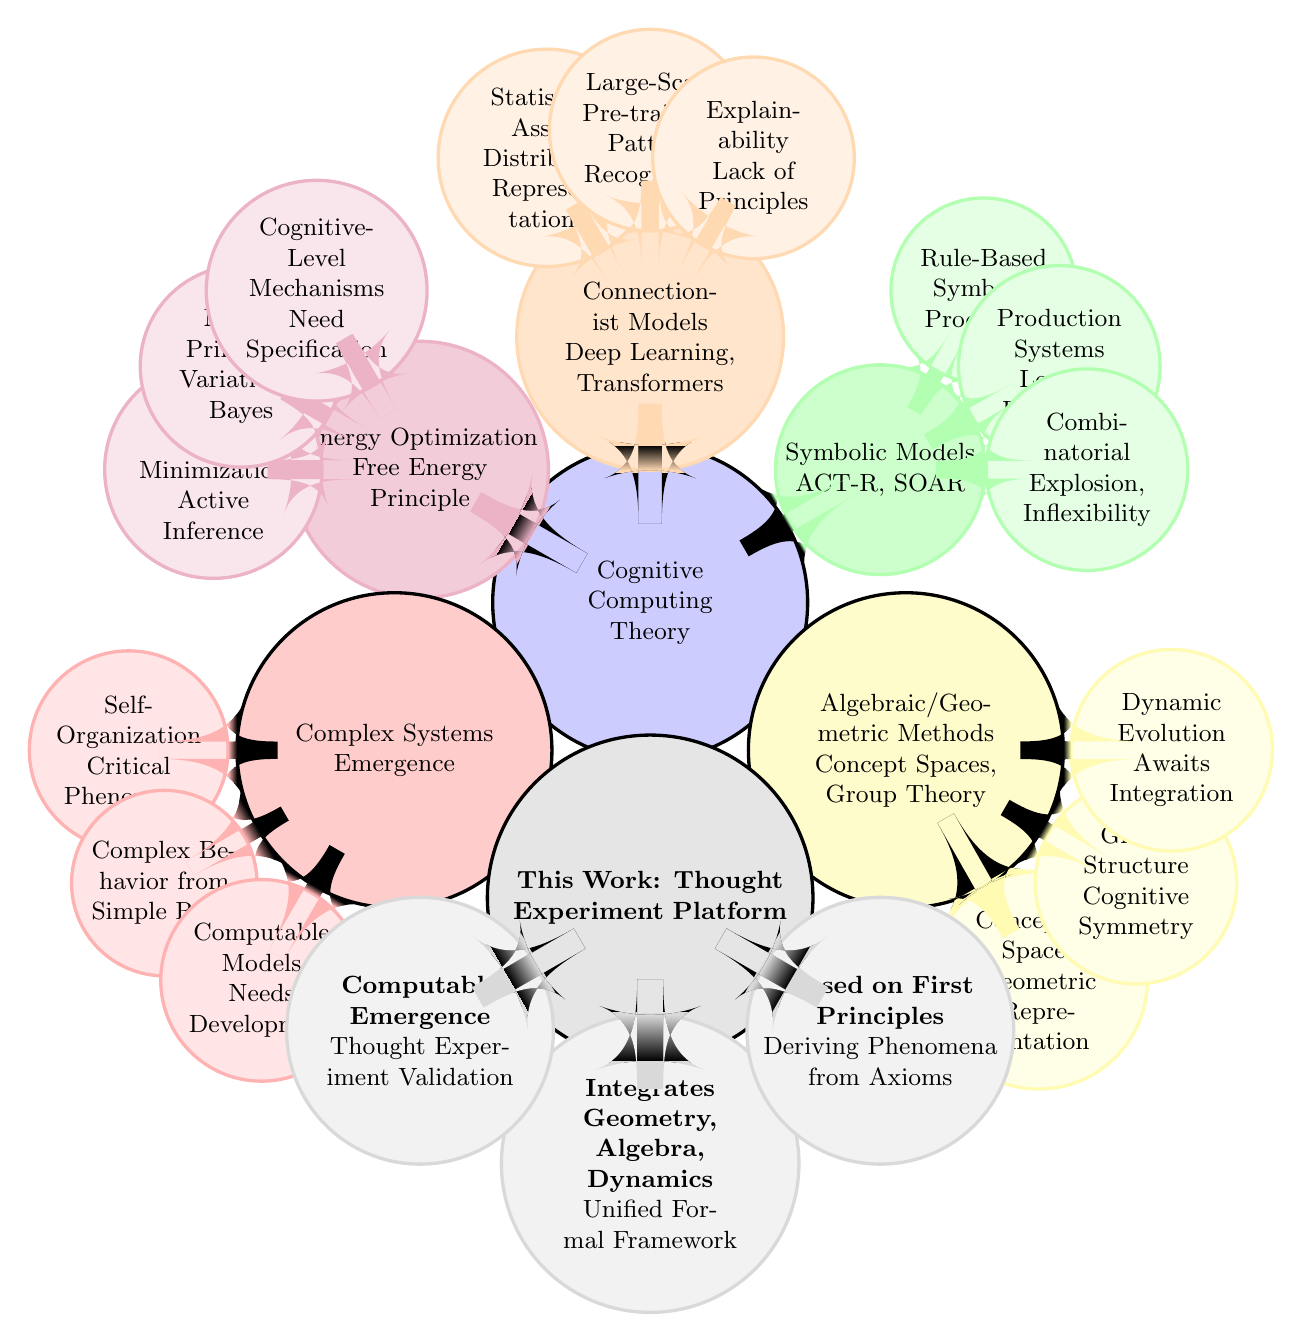
\begin{tikzpicture}[
    scale=0.75,
    mindmap,
    every node/.style={concept, execute at begin node=\hskip0pt, align=center, draw, rectangle, rounded corners=3pt, font=\small},
    level 1 concept/.append style={level distance=4.5cm, sibling angle=120, font=\normalsize\bfseries},
    level 2 concept/.append style={level distance=3.5cm, sibling angle=45, font=\small},
    level 3 concept/.append style={level distance=2.5cm, sibling angle=30, font=\footnotesize},
    text=black
]

% Center: Cognitive Computing Theory
\node[concept, fill=blue!20, text width=2.5cm] {Cognitive Computing\\Theory}
    [clockwise from=0]
    child[concept color=green!30, grow=30] {
        node[concept, fill=green!20, text width=2.5cm] {Symbolic Models\\ACT-R, SOAR}
        child[grow=60] {
            node[concept, fill=green!10, text width=2.0cm] {Rule-Based\\Symbolic Processing}
        }
        child[grow=30] {
            node[concept, fill=green!10, text width=2.0cm] {Production Systems\\Logical Reasoning}
        }
        child[grow=0] {
            node[concept, fill=green!10, text width=2.0cm] {Combinatorial\\Explosion, Inflexibility}
        }
    }
    child[concept color=orange!30, grow=90] {
        node[concept, fill=orange!20, text width=3cm] {Connectionist Models\\Deep Learning, Transformers}
        child[grow=120] {
            node[concept, fill=orange!10, text width=2.0cm] {Statistical Assoc.\\Distributed Representations}
        }
        child[grow=90] {
            node[concept, fill=orange!10, text width=2.0cm] {Large-Scale Pre-training\\Pattern Recognition}
        }
        child[grow=60] {
            node[concept, fill=orange!10, text width=2.0cm] {Explainability\\Lack of Principles}
        }
    }
    child[concept color=purple!30, grow=150] {
        node[concept, fill=purple!20, text width=3cm] {Energy Optimization\\Free Energy Principle}
        child[grow=180] {
            node[concept, fill=purple!10, text width=2.0cm] {Prediction Error Minimization\\Active Inference}
        }
        child[grow=150] {
            node[concept, fill=purple!10, text width=2.0cm] {Neural Principles\\Variational Bayes}
        }
        child[grow=120] {
            node[concept, fill=purple!10, text width=2.0cm] {Cognitive-Level Mechanisms\\Need Specification}
        }
    };

% Second-level branch
\node[concept, fill=yellow!20, text width=3.0cm] at (330:5) {Algebraic/Geometric Methods\\Concept Spaces, Group Theory}
    [clockwise from=270]
    child[concept color=yellow!30, grow=300] {
        node[concept, fill=yellow!10, text width=2.0cm] {Conceptual Spaces\\Geometric Representation}
    }
    child[concept color=yellow!30, grow=330] {
        node[concept, fill=yellow!10, text width=2.0cm] {Group Structure\\Cognitive Symmetry}
    }
    child[concept color=yellow!30, grow=360] {
        node[concept, fill=yellow!10, text width=2.0cm] {Dynamic Evolution\\Awaits Integration}
    };

% Third-level branch
\node[concept, fill=red!20, text width=3.0cm] at (210:5) {Complex Systems\\Emergence}
    [clockwise from=210]
    child[concept color=red!30, grow=180] {
        node[concept, fill=red!10, text width=2.0cm] {Self-Organization\\Critical Phenomena}
    }
    child[concept color=red!30, grow=210] {
        node[concept, fill=red!10, text width=2.0cm] {Complex Behavior from\\Simple Rules}
    }
    child[concept color=red!30, grow=240] {
        node[concept, fill=red!10, text width=2.0cm] {Computable Models\\Needs Development}
    };

% Theoretical Positioning (center bottom)
\node[concept, fill=gray!20, text width=4cm] at (0,-5) {\textbf{This Work: Thought Experiment Platform}}
    child[concept color=gray!30, grow=-90] {
        node[concept, fill=gray!10, text width=3.0cm, align=center] {
            \textbf{Integrates Geometry,\\Algebra, Dynamics}\\
            Unified Formal Framework
        }
    }
    child[concept color=gray!30, grow=-30] {
        node[concept, fill=gray!10, text width=3.0cm, align=center] {
            \textbf{Based on First Principles}\\
            Deriving Phenomena from Axioms
        }
    }
    child[concept color=gray!30, grow=-150] {
        node[concept, fill=gray!10, text width=3.0cm, align=center] {
            \textbf{Computable Emergence}\\Thought Experiment Validation
        }
    };

\end{tikzpicture}
\caption{Theoretical Background Map: Illustrates the core ideas and open questions of major theoretical directions such as symbolism, connectionism, energy optimization, algebraic/geometric methods, and complex systems, along with the positioning of this paper as a thought experiment platform.}
\label{fig:theoretical_background_mindmap}
\end{figure}

Figure \ref{fig:theoretical_background_mindmap} visually presents the core content of this chapter, highlighting the contributions and open problems of existing theories, and clarifying the unique positioning of this paper as a platform for thought experiments.

\section{Axiomatic System of Cognitive Graph Theory: Geometric Description}

This section establishes the geometric axiomatic foundation for cognitive graph theory. We view cognitive states as dynamic networks and introduce energy dynamics as the first principle governing their evolution. Starting from these two fundamental axioms, we observe that the system exhibits a series of derived properties, such as iterability and reversibility. These properties are not arbitrarily defined but are the inevitable consequences of the axioms; they provide a geometric perspective for understanding the continuity and stability of cognitive processes.

\subsection{Basic Axioms}

\textbf{Axiom 1: Cognitive Spacetime (Geometric Formulation)}

There exists a cognitive network $G(V, E, t)$, where:
\begin{itemize}
    \item $V = \{v_1, v_2, \ldots, v_n\}$ is the set of conceptual nodes, where each node $v_i$ represents a basic concept or unit of knowledge.
    \item $E \subseteq V \times V$ is the set of conceptual association edges, where each edge $e_{ij} = (v_i, v_j)$ represents a semantic or functional association between concepts.
    \item $t \in \mathbb{R}^+$ is a continuous time parameter, the network’s topological structure $\Gamma(t)$ and connection weights $w_{ij}(t)$ both evolve over time.
\end{itemize}

This dynamic network constitutes the “stage” on which cognitive activities unfold, with each cognitive state corresponding to a specific geometric configuration of the network. The geometric properties of the network include the degree distribution $P(k)$, the clustering coefficient $C$, path length $L$, modularity $Q$, and others.

\textbf{Axiom 2: Energy Dynamics (Geometric Formulation)}

The evolution of cognitive networks is governed by energy dynamics:

\begin{enumerate}
    \item \textbf{Cognitive Energy Cost Function}: For any edge $e_{ij} \in E$, there exists a cognitive energy cost function:
    \begin{equation}
    E_{ij}(t) = f(\Delta_{ij}, s_{ij}, h_{ij}(t), \Theta)
    \end{equation}
    where $\Delta_{ij}$ is the structural difference between nodes, $s_{ij}$ is the semantic association strength, $h_{ij}(t)$ is the traversal history proficiency, and $\Theta$ is an individual cognitive parameter.

    \item \textbf{Energy consumption evolution mechanism}: The dynamic energy consumption of edges is regulated by historical traversal:
    \begin{equation}
    E_{ij}(t+1) = g(E_{ij}(t), H_{ij}(t), \Theta)
    \end{equation}
    where $H_{ij}(t)$ is the historical traversal record.

    \item \textbf{Optimization objective}: The system’s long-term evolution tends to minimize the global cognitive free energy:
    \begin{equation}
    F(G) = \sum_{e_{ij} \in E} E_{ij} - T \cdot S(G) + R(G)
    \end{equation}
    where $S(G)$ is the network's structural entropy, $T$ is the cognitive temperature parameter, and $R(G)$ is the cognitive resource constraint function.
    \begin{small}
        For brevity, the remainder of this paper often refers to “cognitive energy consumption” as a general term for this free energy, but the mathematical optimization objective is always $F(G)$.
    \end{small}
\end{enumerate}

\begin{figure}[H]
\centering
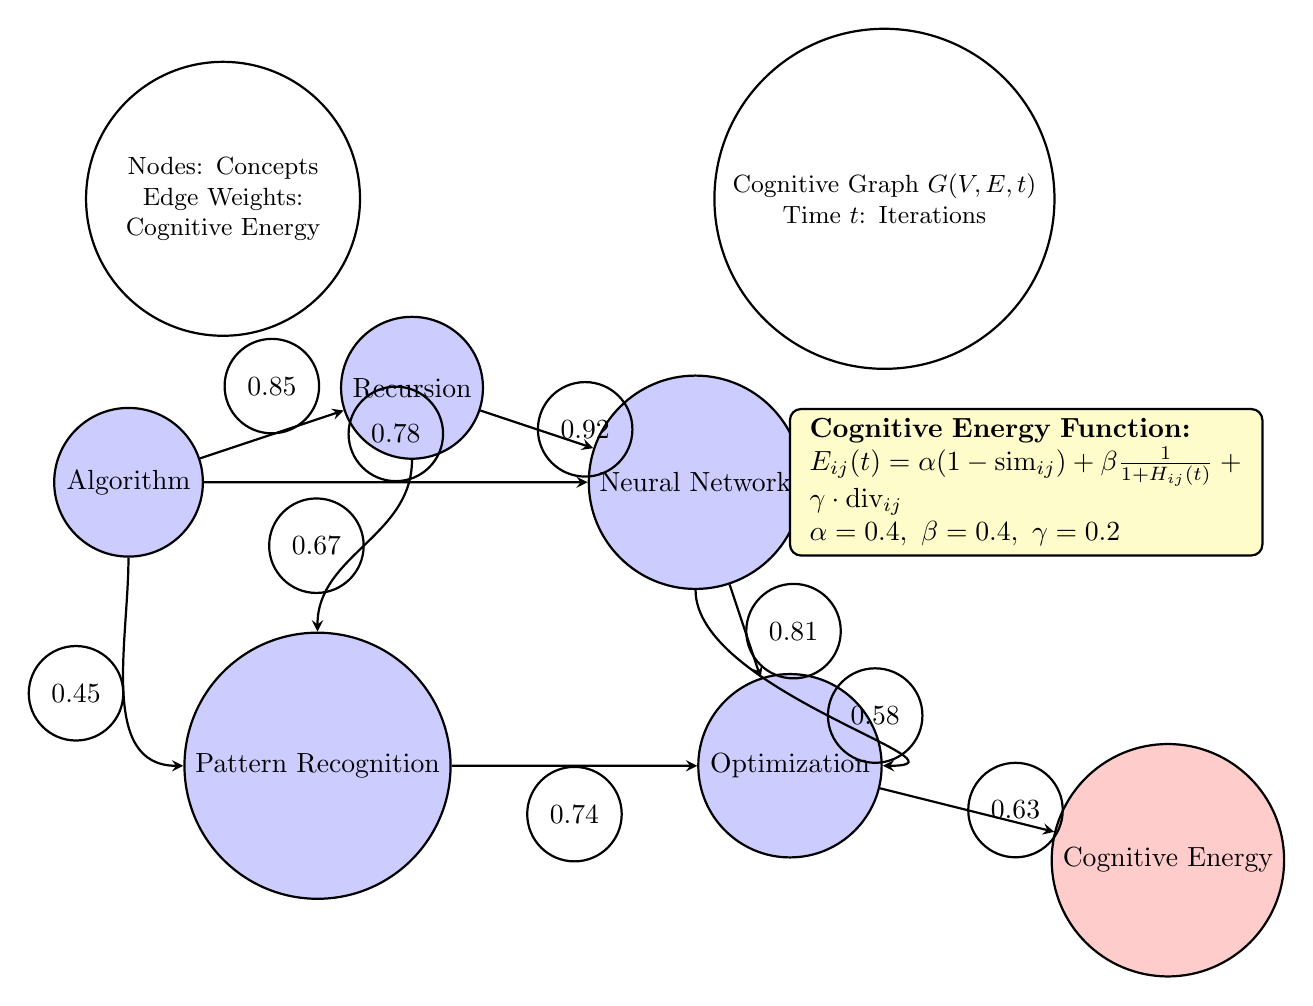
\begin{tikzpicture}[
    scale=1.2,
    every node/.style={circle, draw, minimum size=1.2cm},
    concept/.style={fill=blue!20},
    energy/.style={fill=red!20},
    thick,
    >=stealth
]

\node[concept] (v1) at (-3,1) {Algorithm};
\node[concept] (v2) at (0,2) {Recursion};
\node[concept] (v3) at (3,1) {Neural Network};
\node[concept] (v4) at (-1,-2) {Pattern Recognition};
\node[concept] (v5) at (4,-2) {Optimization};
\node[energy] (v6) at (8,-3) {Cognitive Energy};

\draw[->] (v1) -- node[midway, above] {0.85} (v2);
\draw[->] (v1) -- node[midway, above] {0.78} (v3);
\draw[->] (v2) -- node[midway, right] {0.92} (v3);
\draw[->] (v2) to[out=270, in=90] node[midway, left] {0.67} (v4);
\draw[->] (v3) -- node[midway, right] {0.81} (v5);
\draw[->] (v4) to[out=0, in=180] node[midway, below] {0.74} (v5);
\draw[->] (v5) -- node[midway, right] {0.63} (v6);
\draw[->] (v1) to[out=270, in=180] node[midway, left] {0.45} (v4);
\draw[->] (v3) to[out=270, in=0] node[midway, right] {0.58} (v5);

\node[text width=4cm, align=center, font=\small] at (5,4) {Cognitive Graph $G(V,E,t)$ \\ Time $t$: Iterations};
\node[text width=3cm, align=center, font=\small] at (-2,4) {Nodes: Concepts \\ Edge Weights: Cognitive Energy};

\node[rectangle, draw, rounded corners, fill=yellow!20, minimum width=6cm, minimum height=1.5cm, text width=5.5cm, align=left] at (6.5,1) {
    \textbf{Cognitive Energy Function:} \\
    $E_{ij}(t) = \alpha(1-\text{sim}_{ij}) + \beta\frac{1}{1+H_{ij}(t)} + \gamma\cdot\text{div}_{ij}$ \\
    $\alpha=0.4,\ \beta=0.4,\ \gamma=0.2$
};

\end{tikzpicture}
\caption{Basic Structure of a Cognitive Graph: Nodes represent concepts, edges represent associations between concepts, and edge weights represent cognitive energy consumption. The figure shows concepts like Algorithm, Recursion, Neural Network and their associations. The cognitive energy function decomposes energy into semantic difference, historical familiarity, and structural difference.}
\label{fig:cognitive_graph_structure}
\end{figure}

Note: Graph theory was chosen as the foundational framework because it naturally expresses the context-dependence of concepts—the same node can play different roles (whole or part) in different subgraphs, and cognitive evolution can be simulated through dynamic changes in edges.

\subsection{Geometric Derived Properties}

The following properties are not independent assumptions but necessary corollaries of the above axioms, reflecting the behavioral patterns naturally exhibited by the system under the axioms.

\textbf{Property 1: Iterability (Geometric Formulation)}

The dynamics of cognitive spacetime $G(V,E,t)$ is defined by its own evolution equation:
\begin{equation}
G(t+1) = \Phi(G(t), I(t), \Theta)
\end{equation}
where $\Phi$ is the cognitive evolution operator, $I(t)$ is the external input, and $\Theta$ is the system parameter. This iterative process integrates historical states with new inputs to optimize the network’s geometric structure based on energy dynamics.

\textbf{Property 2: Revertibility (Geometric Formulation)}

Any state $G(t)$ of the system is a complete geometric record of its construction history, which can be formalized as:
\begin{equation}
G(t) = F(A_1, A_2, \ldots, A_t; G(0))
\end{equation}
where $A_i$ is the sequence of historical algorithmic operations, and $G(0)$ is the initial state. This implies that the current geometric state is the “path integral” of its entire history; regressibility is precisely the external manifestation of this path-dependent property, explaining why review enables the rapid restoration of proficiency.

Analysis of the above two properties reveals that both iterability and retrivability are introduced by the time dimension—that is, they are outcomes of dynamics. The originally static graph evolves due to the time dimension, and the evolutionary trajectories of each node concept along the time axis constitute the foundation for cognitive retrivability.

\subsection{Mathematical Formalization}

To enhance the theory’s computability and verifiability, this section provides a mathematical formalization of the core concepts, laying the groundwork for observing and measuring cognitive phenomena in subsequent thought experiments.

\textbf{Cognitive Energy Consumption Function}: To concretize Axiom 2, we define the cognitive energy consumption function of edge $e_{ij}$ at time $t$ as:
\begin{equation}
E_{ij}(t) = \alpha \cdot (1 - \text{sim}(v_i, v_j)) + \beta \cdot \frac{1}{1 + H_{ij}(t)} + \gamma \cdot \text{div}(v_i, v_j)
\label{eq:energy_function}
\end{equation}
where $\text{sim}(v_i, v_j) \in [0,1]$ represents the semantic or structural similarity between nodes, $H_{ij}(t)$ is the number of times the edge has been traversed up to time $t$ (historical familiarity), $\text{div}(v_i, v_j)$ is the structural dissimilarity, and $\alpha, \beta, \gamma$ are weight parameters such that $\alpha + \beta + \gamma = 1$.
\begin{small}
    Note: Equation \eqref{eq:energy_function} is a specific instance of Axiom 2, rather than a fit to real-world observations. This form was chosen because it is intuitive, decomposable, and has precedents in the literature; any energy function satisfying Axiom 2 can drive the system, and this work merely demonstrates the simplest one.
\end{small}

\textbf{Triggering conditions for conceptual compression}: The node set $C = \{v_1, \ldots, v_k\}$ can be compressed into a macro-node $v_C$ if and only if the following holds:
\begin{equation}
\frac{1}{|C|}\sum_{v_i \in C} \overline{E_{i, \text{external}}} > \theta_c \cdot (E_{C, \text{internal}} + \overline{E_{C, \text{external}}})
\label{eq:compression_condition}
\end{equation}
where $\overline{E_{i, \text{external}}}$ is the average energy consumption of a node in $C$ connected to the external environment, $E_{C, \text{internal}}$ is the energy consumption required to maintain the internal structure after compression, $\overline{E_{C, \text{external}}}$ is the average energy consumption of connections to the external environment after compression, and $\theta_c > 1$ is the compression trigger threshold. This inequality indicates that when the average external energy consumption required to maintain a dispersed structure exceeds the threshold of the total energy consumption after compression, compression becomes the energy-optimal solution.

\subsection{Cluster Compression Potential: A Continuous Metric}
\label{subsec:compression_potential}

To more precisely characterize the intrinsic energy properties of the concept of compression, we introduce a continuous metric—the cluster compression potential. For any candidate node set $C \subseteq V$, we define its compression potential as:
\begin{equation}
\Phi(C) = \frac{\overline{E}_{\text{internal}}(C)}{\overline{E}_{\text{external}}(C)}
\label{eq:compression_potential}
\end{equation}
where $\overline{E}_{\text{internal}}(C)$ is the average cognitive energy cost of all edges within set $C$, and $\overline{E}_{\text{external}}(C)$ is the average cognitive energy cost of all edges between nodes in $C$ and external nodes ($V \setminus C$). The smaller the value of $\Phi(C)$, the more tightly connected the cluster is internally (low energy cost) and the more loosely connected it is externally (high energy cost); therefore, the greater the expected energy savings from compressing this cluster.

The compression potential is a purely observational metric; it does not influence the system’s evolutionary decisions but is used solely for post-hoc analysis of the statistical characteristics of clusters actually compressed by the system. It is essentially equivalent to the compression trigger condition defined in Section 3.3 (Equation \ref{eq:compression_condition})—the compression potential reflects the energy consumption ratio between the interior and exterior of a cluster, while the trigger condition represents the specific manifestation of this ratio exceeding a certain threshold. The introduction of the compression potential enables us to examine the quality of compression behavior in a continuous and objective manner, and provides a quantitative basis for the scale effect analysis in Section 7.3.

\subsection{Geometric Theory of Cognitive Permutation}

As an operational realization of energy dynamics, system evolution relies on two fundamental cognitive traversal modes, which correspond to different modes of motion in cognitive space.

\textbf{Definition 3.5.1 (Hard Perpetual Motion)}: The system performs precise, efficient cognitive operations along existing low-energy-cost paths; these paths exhibit high determinism and low energy consumption, serving the consolidation and application of knowledge. Geometrically, this manifests as motion on a known low-dimensional manifold.

\textbf{Definition 3.5.2 (Soft Perpetual Motion)}: The system searches for new or weakly correlated paths at a higher exploratory cost; these paths exhibit strong randomness and higher energy consumption, serving the exploration and innovation of knowledge. Geometrically, this manifests as exploration in high-dimensional or unknown regions.

\subsection{Contextual Assumptions}

The theoretical framework and experimental design of this study are based on a clear premise: all cognitive activities occur within a \textbf{single static context}. A single static context refers to a situation where, within the same cognitive scenario, the network structure formed by conceptual nodes and their associative edges remains unchanged despite contextual shifts, and the entire evolutionary process unfolds on a fixed “cognitive stage.” This is analogous to the “isolated system” assumption used in physics when studying ideal gases—although real gases always exchange energy with the external environment, the simplification of an isolated system allows us to first uncover the fundamental laws governing core variables such as pressure and temperature.

Real-world cognitive processes are always highly context-dependent, but if multi-context mechanisms are introduced at the outset of modeling, we face the dual complexity of both the dynamic evolution of conceptual representations and context switching, making it difficult to clearly isolate the role of the energy minimization principle itself. Therefore, we first establish a foundational model within a single static context, focusing on observing how the core driving force of “cognitive energy minimization” shapes cognitive structures. Once the fundamental laws are clarified, we will gradually incorporate the contextual dimension.

Although we currently adopt a static context assumption, graph theory itself provides interfaces for modeling dynamic contexts: context nodes can be introduced, dynamic edge weights can be context-modulated, and context evolution operators can be incorporated. Thus, the static context model established in this work represents the first step toward dynamic context-based cognitive simulation.

\section{Algebraic Structures in Cognitive Graph Theory: Group Description}

In the previous section, we characterized cognitive states as dynamic networks from a geometric perspective. This section attempts to introduce algebraic tools to provide a more structured description of cognitive operations. Group theory, as a mathematical language for studying symmetry and transformations, can help us understand the combinatorial relationships, reversibility, and possible conserved quantities among cognitive operations. It should be noted that the algebraic structure proposed here is a formalization attempt, aiming to provide an abstract mathematical perspective for subsequent cognitive dynamics analysis, rather than asserting that real cognition strictly follows all group axioms.

\subsection{Algebraic Systems of Cognitive Operations}

To provide a richer mathematical description for cognitive graph theory, we consider using algebraic structures to characterize the interrelationships among basic cognitive operations.

Let $\cognitivespace$ be the set of all possible cognitive states, i.e., $\cognitivespace = \{G(V,E,t) | t \in \mathbb{R}^+\}$. Basic cognitive operations include traversal $\tau$, learning $\lambda$, forgetting $\phi$, compression $\kappa$, and transfer $\mu$. The set of these operations forms a semigroup under composition: the composition of any two operations remains a cognitive operation, and composition satisfies the associative law (though not necessarily the commutative law). The identity element corresponds to the “empty operation” (leaving the state unchanged). This structure provides an algebraic foundation for understanding the combinatorial properties of cognitive processes.

\begin{figure}[H]
\centering
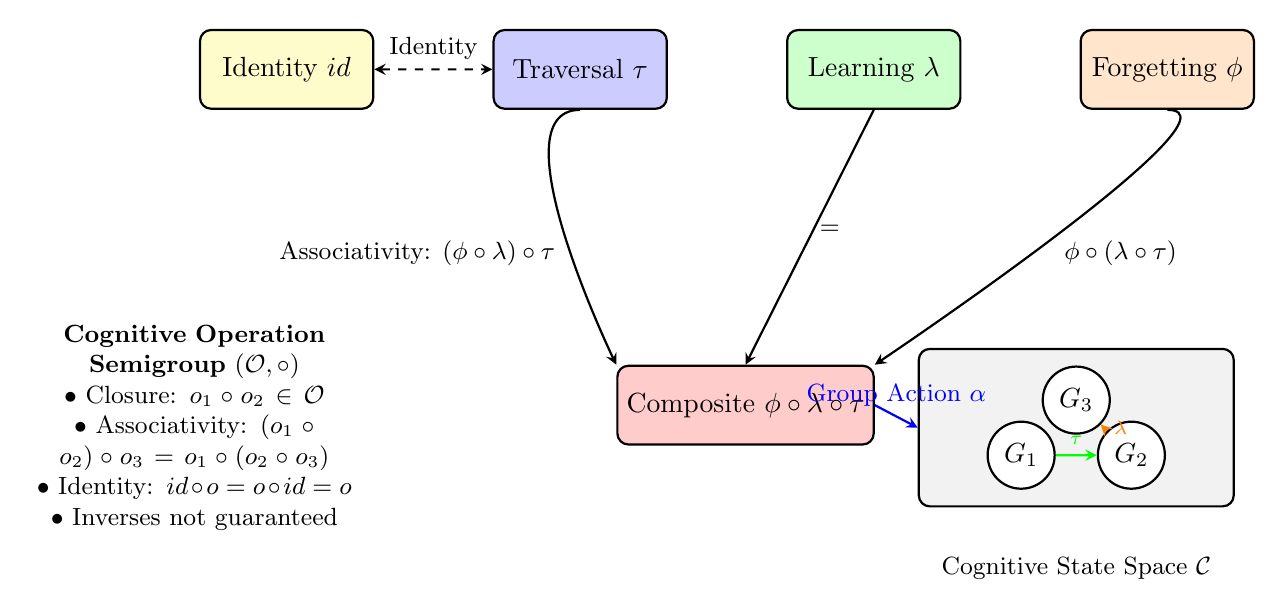
\begin{tikzpicture}[
    scale=0.70,
    operation/.style={rectangle, draw, rounded corners, minimum width=2.2cm, minimum height=1cm, align=center},
    op1/.style={fill=blue!20},
    op2/.style={fill=green!20},
    op3/.style={fill=orange!20},
    result/.style={fill=red!20},
    space/.style={rectangle, draw, rounded corners, fill=gray!10, minimum width=4cm, minimum height=2cm},
    thick,
    >=stealth,
    node distance=1.5cm
]

\node[operation, op1] (tau) at (0,3) {Traversal $\tau$};
\node[operation, op2, right=of tau] (lambda) {Learning $\lambda$};
\node[operation, op3, right=of lambda] (phi) {Forgetting $\phi$};

\node[operation, result, below=2cm of lambda] (composite) at (3,0.5) {Composite $\phi\circ\lambda\circ\tau$};

\draw[->, thick] (tau.south) .. controls (tau.south west) and (composite.north west) .. 
    node[midway, left, font=\small, yshift=-0.2cm] {Associativity: $(\phi\circ\lambda)\circ\tau$} (composite.north west);
\draw[->, thick] (lambda.south) .. controls (lambda.south) and (composite.north) .. 
    node[midway, right, font=\small, yshift=0.1cm] {$=$} (composite.north);
\draw[->, thick] (phi.south) .. controls (phi.south east) and (composite.north east) .. 
    node[midway, right, font=\small, yshift=-0.2cm] {$\phi\circ(\lambda\circ\tau)$} (composite.north east);

\node[operation, fill=yellow!20, left=of tau] (id) {Identity $id$};
\draw[<->, dashed, thick] (id) -- node[midway, above, font=\small] {Identity} (tau);

\node[space] (space) at (9, -3.5) {};
\node[circle, draw, fill=white] (state1) at (8, -4) {$G_1$};
\node[circle, draw, fill=white] (state2) at (10, -4) {$G_2$};
\node[circle, draw, fill=white] (state3) at (9, -3) {$G_3$};

\draw[->, thick, blue] (composite.east) -- (space.west) 
    node[midway, above, font=\small] {Group Action $\alpha$};
\draw[->, thick, green] (state1) -- node[midway, above, font=\scriptsize] {$\tau$} (state2);
\draw[->, thick, orange] (state2) -- node[midway, right, font=\scriptsize] {$\lambda$} (state3);

\node[text width=4cm, align=center, font=\small] at (-7, -3.5) {
    \textbf{Cognitive Operation Semigroup $(\mathcal{O},\circ)$} \\
    $\bullet$ Closure: $o_1\circ o_2 \in \mathcal{O}$ \\
    $\bullet$ Associativity: $(o_1\circ o_2)\circ o_3 = o_1\circ(o_2\circ o_3)$ \\
    $\bullet$ Identity: $id\circ o = o\circ id = o$ \\
    $\bullet$ Inverses not guaranteed
};

\node[below=0.5cm of space, font=\small] {Cognitive State Space $\mathcal{C}$};

\end{tikzpicture}
\caption{Algebraic structure of cognitive operations: Basic cognitive operations form a semigroup satisfying closure and associativity. The figure illustrates the composition of the three operations—traversal $\tau$, learning $\lambda$, and forgetting $\phi$—as well as their effects on the cognitive state space $\mathcal{C}$ via the group action $\alpha$.}
\label{fig:cognitive_semigroup}
\end{figure}

\subsection{Cognitive Symmetry and Invariance}

In cognitive networks, certain transformations may preserve the system's key properties; this invariance can be described using the concept of symmetry groups. Let $\cognitivegroup$ be the group of transformations that preserve certain properties of a cognitive network; this can be referred to as the cognitive symmetry group. It may contain subgroups such as the concept isomorphism group $\text{Aut}(V)$ (permutations that preserve the semantic structure of concepts), the structural homology group $\pi_1(\cognitivespace)$ (which characterizes the topological structure of the cognitive space), and the energy conservation group $\text{Iso}(E)$ (isometric transformations that preserve global energy), among others.

In physical systems, continuous symmetries often correspond to conserved quantities (Noether’s theorem). In cognitive systems, we can also attempt to find similar correspondences: time-translation symmetry corresponds to the tendency toward cognitive energy conservation, concept permutation symmetry corresponds to the relative stability of structural entropy, and scale transformation symmetry with the preservation of fractal dimension. Such correspondences exhibit certain trends in experiments (see Appendix A), but they serve more as an inspirational perspective rather than strict mathematical theorems.

\subsection{Group Actions on Cognitive Operations}

Symmetry groups can act on the cognitive state space, and this action can be described using the concept of group action. The group action $\alpha: \cognitivegroup \times \cognitivespace \rightarrow \cognitivespace$ satisfies the identity element property and is compatible with group multiplication. For a given state $G$, its orbit $O_G = \{\alpha(g, G) | g \in \cognitivegroup\}$ represents all states reachable via symmetry transformations; the stabilizer $\text{Stab}(G) = \{g \in \cognitivegroup | \alpha(g, G) = G\}$ denotes the symmetric operations that leave $G$ invariant. For finite groups, the size of the orbit and the size of the stabilizer satisfy $|O_G| = |\cognitivegroup|/|\text{Stab}(G)|$. In cognitive networks, due to individual differences and historical dependencies, symmetry is typically low, and orbits are often small or even consist solely of the individual itself.

\subsection{Lie Group Descriptions of Cognitive Evolution}

For continuous-time evolution, one may attempt to describe cognitive dynamics using the language of Lie groups. Let $\cognitivegroup$ be a Lie group whose Lie algebra $\mathfrak{g}$ has generators corresponding to basic cognitive operations, such as the energy optimization operator $\energyoperator$, the concept compression operator $\compressionoperator$, and the principle transfer operator $\migrationoperator$. The evolution of cognitive states can be described by equations on the Lie group:
\begin{equation}
\frac{dG(t)}{dt} = A(t)G(t), \quad A(t) \in \mathfrak{g}
\end{equation}
This equation expresses cognitive dynamics as motion on a Lie group, providing a mathematical framework for analyzing the continuous changes in cognitive processes. In practical computations, we use a discrete approximation to simulate this process.

\subsection{The Cognitive Significance of Algebraic Structures}

The introduction of algebraic structures facilitates a formal description of cognitive processes: closure suggests the self-contained nature of cognitive operations; associativity corresponds to the coherence of thought processes; the identity element corresponds to invariant operations such as “maintaining attention”; and the existence of inverses reflects the (ir)reversibility of cognitive processes. These algebraic properties provide a computable mathematical language for cognitive operations, but they do not participate in the system’s decision-making or evolution—evolution remains independently driven by energy dynamics.

\section{Verification of the Computability of the Algebraic Framework}
\label{sec:algebraic_experiments}

To test the operational feasibility of the algebraic framework proposed in Section 4 within a thought-experiment setting, we designed five sets of computational observations, targeting the cognitive operation semigroup, Noetherian correspondences, the orbit-stabilizer theorem, the Lie group evolution framework, and the extensibility of the algebraic method, respectively. Detailed experimental setup, data, and analysis are provided in Appendix A. This section reports only the core observational conclusions.

\textbf{Cognitive Operation Semigroup}: In combination tests of 13 basic cognitive operations, all operation compositions satisfied the associative law, indicating that the set of cognitive operations forms a semigroup under composition. This observation provides algebraic support for the coherence and composability of cognitive processes.

\textbf{Noetherian Correspondence Trend}: Across three cognitively structured networks, global cognitive energy, structural entropy, and fractal dimension all exhibited high stability under symmetric transformations (relative changes < 1\%), suggesting the existence of conservation laws similar to those in physics. The network isomorphism number is 1 in all cases (only the identity mapping), reflecting the individual uniqueness and low symmetry of cognitive systems.

\textbf{Applicability of the Orbit-Stabilizer Theorem}: Due to the highly personalized nature of cognitive networks, the cognitive symmetry group contains only the identity map, and the orbit-stabilizer relation holds trivially ($1 = 1/1$). This trivial verification indirectly confirms the characteristic lack of mathematical symmetry in cognitive systems due to differences in learning history and weights.

\textbf{Feasibility of the Lie Group Evolution Framework}: By conducting continuous evolution simulations using three different combinations of generators (energy optimization-dominated, concept compression-dominated, and principle transfer-dominated), we observed energy consumption reductions of 34.7\%, 14.7\%, and 12.4\%, respectively. The strategy dominated by the energy optimization operator proved most effective, while principle transfer, despite yielding a smaller reduction in energy consumption, laid the foundation for creative connections.

\textbf{Scalability of the Algebraic Approach}: In networks ranging from 5 to 15 nodes, all algebraic operations took less than 0.1 seconds, meeting real-time analysis requirements. The factorial complexity ($O(n!)$) of symmetry detection limits large-scale applications, but this can be optimized through heuristic algorithms.

These observations indicate that algebraic tools such as group theory can provide a formal description of cognitive processes and are computationally feasible in medium-sized networks. The algebraic framework not only provides a mathematical language for the combination and transformation of cognitive operations but also opens new perspectives for understanding the structural conservation, evolutionary patterns, and individual differences of cognitive systems. For detailed experimental data, algorithm implementations, and a list of case studies, please refer to Appendix A.

\section{Emergence Mechanisms Driven by Energy Dynamics}

The first two sections established formal frameworks for cognitive processes from geometric and algebraic perspectives, respectively. In this section, we turn our attention to the dynamic evolution of the system to observe what macroscopic behavioral patterns cognitive networks spontaneously generate under the core driving force of energy minimization. We will see that “concept compression” and “first-principles transfer” are not pre-programmed by an external designer, nor are they “operations” actively executed by the system; rather, they are typical phenomena naturally emerging from energy optimization that we capture during the observation process. These emergent patterns provide a computable window of observation for understanding how knowledge is organized and the origins of creative thinking.

It is important to note that the descriptions presented in this section are not “generative rules” for compression or transfer phenomena, but rather diagnostic tools used to “observe” and “record” these macroscopic patterns during the system’s evolution. The true driving force behind these phenomena remains the energy dynamics postulate defined in Section 3—the system merely continuously traverses and updates its energy consumption, while we, as observers, identify macroscopic structures consistent with compression or transfer characteristics from changes in the network’s energy distribution.

\subsection{Conceptual Compression: Emergence as Network Reconstruction}

As a complex system governed by the principles of energy dynamics, cognitive spacetime spontaneously exhibits a macroscopic behavior we term “conceptual compression.” From a geometric perspective, conceptual compression is a self-organizing process within localized regions of cognitive space; from an algebraic perspective, it can be viewed as a manifestation of symmetry breaking and the formation of order parameters.

\textbf{Theoretical Description}: When a group of conceptual nodes is highly semantically similar, exhibits extremely low energy consumption among themselves, and displays high energy consumption in connections with external nodes, treating this group as a single entity (i.e., “compressing” into a macroscopic node) can significantly reduce global energy consumption. This structural reorganization is a natural outcome of the system’s pursuit of energy minimization.

\textbf{Observations}: In the code implementation, we did not design any “active compression” instructions. The system merely updates edge energy costs according to the rules of energy dynamics, while we, as observers, periodically scan the network to detect whether a set of nodes exists that are tightly connected to one another (low energy cost) and exhibit a certain degree of synergy in their connections to external nodes. When a set of nodes satisfying these conditions is detected, we record a “concept compression” event. In other words, compression is an observed phenomenon, not a command executed by the system.

\textbf{Description 6.1.1 (Geometric Characteristics of Conceptual Compression)}: Let there exist a set of nodes $C = \{v_1, v_2, \ldots, v_k\} \subset V$. If the following characteristic is observed:
\begin{enumerate}
    \item \textbf{Structural similarity}: $\forall v_i, v_j \in C, \text{sim}(v_i, v_j) > \theta_s$
    \item \textbf{Energy synergy}: $\exists v_c \in V, \forall v_i \in C, E_{c,i} < \overline{E} - \delta_E$
    \item \textbf{Traversal synchrony}: $v_i$ and $v_j \in C$ are frequently co-activated in the traversal history
\end{enumerate}
the system often undergoes network restructuring, creating a macroscopic node $v_C$ to encapsulate the microstructure $C$. This restructuring can be viewed as an economical way for the system to handle high-frequency co-occurrence patterns.

\textbf{Observation 6.1.2 (Algebraic Meaning of Concept Compression)}: From an algebraic perspective, the concept compression operation $\kappa_C$ can be viewed as a subgroup action of the cognitive symmetry group $\cognitivegroup$, which aids in understanding the combinatorial relationships among compression operations.

\begin{figure}[H]
\centering
\vspace{0.3cm}
\begin{subfigure}[b]{0.45\textwidth}
\centering
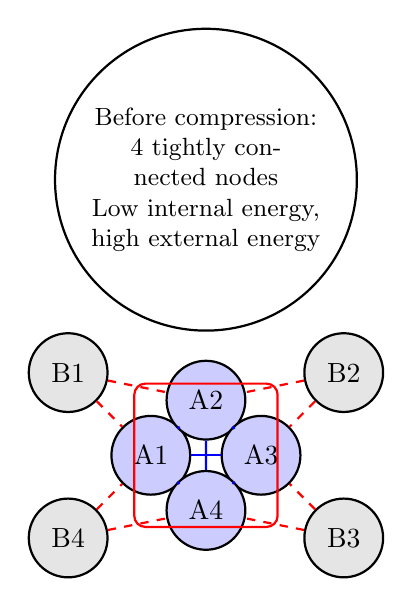
\begin{tikzpicture}[
    scale=0.7,
    every node/.style={circle, draw, minimum size=1cm},
    cluster1/.style={fill=blue!20},
    cluster2/.style={fill=green!20},
    other/.style={fill=gray!20},
    thick
]

% Before compression: 4 tightly connected nodes
\node[cluster1] (a1) at (0,0) {A1};
\node[cluster1] (a2) at (1,1) {A2};
\node[cluster1] (a3) at (2,0) {A3};
\node[cluster1] (a4) at (1,-1) {A4};

% External nodes
\node[other] (b1) at (-1.5,1.5) {B1};
\node[other] (b2) at (3.5,1.5) {B2};
\node[other] (b3) at (3.5,-1.5) {B3};
\node[other] (b4) at (-1.5,-1.5) {B4};

% Internal connections (low energy)
\draw[blue, thick] (a1) -- (a2);
\draw[blue, thick] (a1) -- (a3);
\draw[blue, thick] (a1) -- (a4);
\draw[blue, thick] (a2) -- (a3);
\draw[blue, thick] (a2) -- (a4);
\draw[blue, thick] (a3) -- (a4);

% External connections (high energy)
\draw[red, dashed] (b1) -- (a1);
\draw[red, dashed] (b1) -- (a2);
\draw[red, dashed] (b2) -- (a2);
\draw[red, dashed] (b2) -- (a3);
\draw[red, dashed] (b3) -- (a3);
\draw[red, dashed] (b3) -- (a4);
\draw[red, dashed] (b4) -- (a4);
\draw[red, dashed] (b4) -- (a1);

\node[text width=3cm, align=center, font=\small] at (1,5.0) {Before compression: \\ 4 tightly connected nodes \\ Low internal energy, high external energy};

\draw[red, thick, rounded corners] (-0.3,-1.3) rectangle (2.3,1.3);

\end{tikzpicture}
\caption{Before compression: dispersed structure}
\end{subfigure}
\hspace{0.5cm}
\begin{subfigure}[b]{0.45\textwidth}
\centering
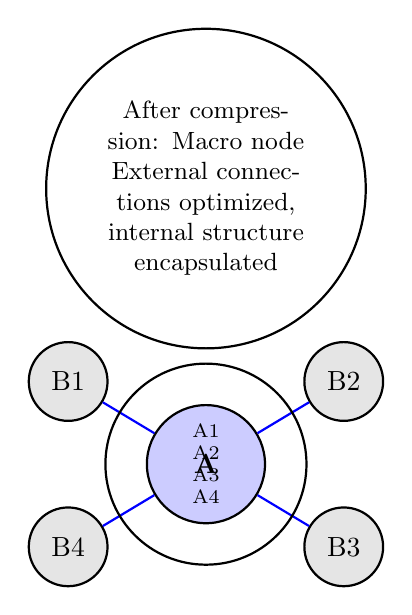
\begin{tikzpicture}[
    scale=0.7,
    every node/.style={circle, draw, minimum size=1cm},
    macro/.style={fill=blue!20, minimum size=1.5cm},
    other/.style={fill=gray!20},
    thick
]

% Macro node after compression
\node[macro] (macro) at (1,0) {\textbf{A}};

% External nodes
\node[other] (b1) at (-1.5,1.5) {B1};
\node[other] (b2) at (3.5,1.5) {B2};
\node[other] (b3) at (3.5,-1.5) {B3};
\node[other] (b4) at (-1.5,-1.5) {B4};

% External connections (optimized)
\draw[blue, thick] (b1) -- (macro);
\draw[blue, thick] (b2) -- (macro);
\draw[blue, thick] (b3) -- (macro);
\draw[blue, thick] (b4) -- (macro);

\node[text width=2cm, align=center, font=\scriptsize] at (1,0) {A1 \\ A2 \\ A3 \\ A4};

\node[text width=3cm, align=center, font=\small] at (1,5.0) {After compression: Macro node \\ External connections optimized, internal structure encapsulated};

\end{tikzpicture}
\caption{After compression: Macro-structure}
\end{subfigure}
\vspace{0.5cm}

\caption{Schematic diagram of the conceptual compression process: When the node set $C=\{A1,A2,A3,A4\}$ satisfies the compression conditions, the system compresses these four closely connected nodes into a single macroscopic node $A$. (a) Before compression: Each of the four nodes has high-energy-consumption connections with external nodes; (b) After compression: Macro-node $A$ integrates the functions of the four nodes, retaining only optimized external connections, significantly reducing cognitive energy expenditure. The condition for detecting one instance of “concept compression” is: $\frac{1}{|C|}\sum_{v_i\in C}\overline{E_{i,\text{external}}} > \theta_c\cdot(E_{C,\text{internal}}+\overline{E_{C,\text{external}}})$.}
\label{fig:compression_process}
\end{figure}

\subsection{Cognitive Rationality Analysis of Concept Compression}

The concept compression phenomena observed in experiments—including apparent “problems” such as overgeneralization, large semantic spans, and redundant detection—actually reveal a profound correspondence with the laws of human cognition. Overgeneralization mimics a common phenomenon in children’s language acquisition; connections with large semantic spans embody metaphorical thinking and creative analogy; and redundant compression reflects the necessary process of memory consolidation. Together, these phenomena indicate that naturally emerging cognitive systems generate pattern-generation strategies analogous to biological cognition, thereby demonstrating the biological rationality of emergent mechanisms—which reproduce the fundamental dynamics of cognitive evolution.

\subsection{First-Principles Transfer: Emergence as Optimal Path Search}

The essence of first-principles transfer lies in the system’s intelligent route selection driven by energy dynamics. From an algebraic perspective, it can be viewed as the connection of orbits under group action; from a geometric perspective, it is the discovery of geodesics in cognitive space. Similar to conceptual compression, transfer is a phenomenon we observe rather than an instruction actively executed by the system—the system merely continuously updates the energy cost of edges, and we identify those paths that significantly reduce energy costs by connecting through principle nodes.

\textbf{Description 6.3.1 (Geometric Characteristics of Principle-Based Transfer)}: For nodes $v_a, v_b \in V$, if the energy cost of a direct connection $E_{ab}$ is too high, the system often seeks an intermediary node $v_z$ such that:
\begin{equation}
E_{az} + E_{zb} < E_{ab} - \Delta_{\text{threshold}}
\end{equation}
where $v_z$ is typically a structurally robust, well-connected principle node.

\textbf{Observation 6.3.2 (Algebraic Meaning of Transfer Paths)}: Principle transfer paths can be viewed as a coset of the cognitive symmetry group $\cognitivegroup$, which aids in understanding the symmetry of transfer paths.

Taking the property that sound can be decomposed into a superposition of different frequencies (Fourier transform/spectral analysis), and frequency-domain processing in image examples, their evolutionary processes in the macro-cognitive graph can be schematized as follows:
\begin{figure}[H]
\centering
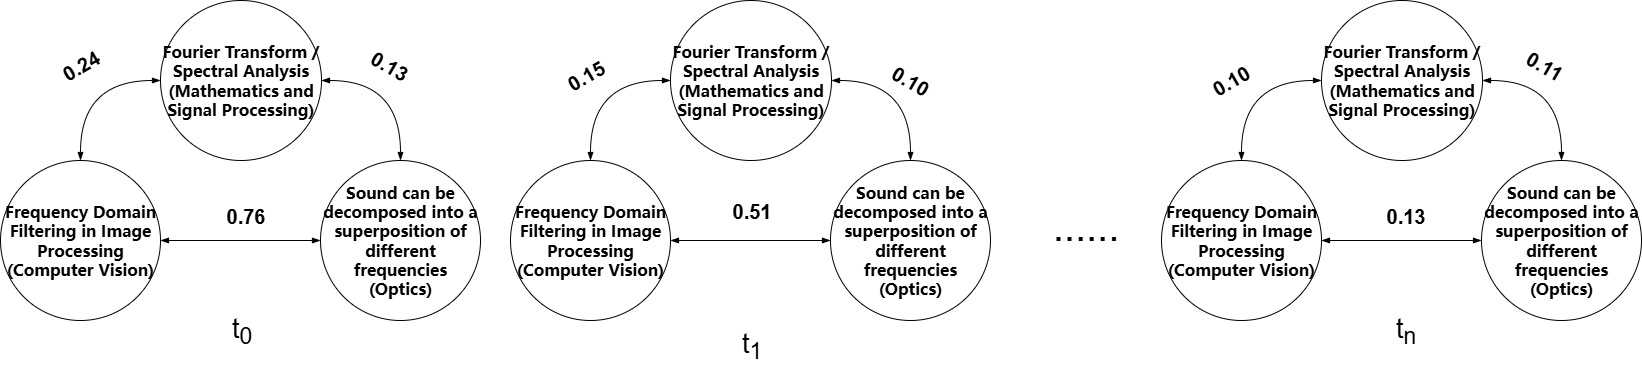
\includegraphics[width=0.95\textwidth]{fig5_migration.png}
\caption{Theoretical schematic of principle-based transfer: Connecting concepts across different domains (e.g., sound $\rightarrow$ Fourier transform $\rightarrow$ image processing) through the core principle node “transform,” forming a low-energy-consumption pathway. The direction of the arrows in the figure indicates the flow of energy; the “transform” node acts as a bridge to facilitate cross-domain knowledge transfer, illustrating the central role of first principles in creative thinking.}
\label{fig:migration_theory}
\end{figure}

\subsection{Analysis of the Cognitive Rationality of First-Principles Transfer}

The phenomena of first-principles transfer observed in experiments, including seemingly “irrational” connections, reveal a profound correspondence with the laws of human creative thinking. Individual threshold differences simulate the diversity of cognitive styles, cross-domain transfer embodies the core mechanism of analogical thinking, the bridging role of principle nodes resembles “cognitive primitives,” and seemingly irrational transfers may simulate the cognitive processes behind human insight and inspiration. Together, these mechanisms form the dynamical basis of creative thinking.

\subsection{Phase Transition Phenomena in Cognitive States}

In the framework of energy dynamics, cognitive systems exhibit typical phase transition behavior. When system parameters (such as cognitive temperature $T$, learning rate $\eta$, etc.) cross certain critical thresholds, the behavior of the cognitive system undergoes a qualitative change. In our experiments, we observed a distinct phase transition occurring after approximately 3,000 iterations, marking a shift from a phase dominated by local optimization to one dominated by global restructuring—a transition that corresponds to the concentrated emergence of creative insights. This phase transition phenomenon can be described using renormalization group theory and provides a window into understanding the fundamental shifts in cognitive strategies.

\section{Experimental Design and Results Analysis}

\subsection{Experimental Setup and Parameter Configuration}

The experiment employed a parallel design of four systems of different scales, running on networks of 51, 71, 91, and 111 cross-domain concepts, respectively, to observe the behavioral patterns of cognitive systems under environments of varying knowledge complexity. These scales represent knowledge spaces ranging from relatively simple to highly complex, simulating differences in domain-specific knowledge density or individual knowledge breadth.

\textbf{Network Construction Strategy}: Concepts span multiple disciplines including physics, mathematics, computer science, artificial intelligence, cognitive science, neuroscience, and philosophy. A meta-structure mapping (\texttt{META\_STRUCTURE\_MAP}) was introduced to classify specific concepts into abstract meta-categories such as “information,” “geometry,” “motion,” “method,” and “energy,” thereby enhancing the system’s sensitivity to cross-domain conceptual associations.

\textbf{Unified Threshold Settings}: To ensure comparability across experiments of varying scales, all experiments employ a unified cognitive emergence threshold (compression synergy threshold 0.76, transfer efficiency threshold 0.35, cluster cohesion threshold 0.7, minimum connection strength 0.5), with a learning rate of 0.85, cognitive temperature $T = 1.0$, and 10,000 iterations. See Table \ref{tab:multi_scale_config} for detailed parameters.

\begin{table}[H]
\small
\centering
\caption{Experimental parameter configurations for four scales}
\label{tab:multi_scale_config}
\begin{tabular}{lcccc}
\toprule
\textbf{Parameter} & \multicolumn{4}{c}{\textbf{Concept Scale}} \\
\cmidrule(lr){2-5}
& 51 & 71 & 91 & 111 \\
\midrule
Number of concept nodes & 51 & 71 & 91 & 111 \\
Initial number of edges & 242 & 469 & 801 & 1224 \\
Semantic similarity threshold & 0.08 & 0.08 & 0.08 & 0.08 \\
Compression synergy threshold & 0.76 & 0.76 & 0.76 & 0.76 \\
Migration efficiency threshold & 0.35 & 0.35 & 0.35 & 0.35 \\
Learning rate & 0.85 & 0.85 & 0.85 & 0.85 \\
Cognitive Temperature $T$ & 1.0 & 1.0 & 1.0 & 1.0 \\
Number of iterations & 10,000 & 10,000 & 10,000 & 10,000 \\
Number of individuals & 3 & 3 & 3 & 3 \\
\bottomrule
\end{tabular}
\end{table}

\subsection{Analysis of Scale Effects in Energy Consumption Optimization}

The energy optimization performance of the naturally emergent model across four scales is shown in Table \ref{tab:multi_scale_energy}. As the number of concepts increases, the magnitude of energy reduction decreases systematically; however, even with 111 concepts, a 47.9\% reduction is still achieved, demonstrating the adaptability of the energy minimization principle across different knowledge densities.

\begin{table}[h]
\centering
\caption{Energy consumption optimization of the self-organizing model across four scales}
\label{tab:multi_scale_energy}
\begin{tabular}{lcc}
\toprule
\textbf{Conceptual Scale} & \textbf{Energy Savings} & \textbf{Reduction Trend} \\
\midrule
51 Concept & 86.9\% & Baseline \\
71 Concept & 72.3\% & -14.6\% \\
91 Concept & 61.4\% & -25.5\% \\
111 Concepts & 47.9\% & -39.0\% \\
\bottomrule
\end{tabular}
\end{table}

As a comparison, the predefined algorithmic model incorporating external intervention rules (see Appendix B) achieved energy reductions of 22.8\%, 15.5\%, 12.2\%, and 7.6\% at the same scales, respectively, exhibiting a much steeper decline in performance (a 67.1\% drop). This comparison suggests that self-organizing mechanisms based on energy minimization possess greater robustness when facing increasing complexity.

\subsection{Scale-Adaptive Patterns of Emergent Phenomena}
\label{sec:scale_dependent_emergence}

This section analyzes the patterns of cognitive emergence phenomena as network scale changes from multiple perspectives, including the number of compressions, the number of transitions, and the compression potential. Key metrics are shown in Table \ref{tab:scale_dependent_emergence}.

\subsubsection{Macroscopic Statistics of Compression and Migration}

Experiments observed systematic changes in cognitive emergence patterns with network scale; key metrics are shown in Table \ref{tab:scale_dependent_emergence}.

\begin{table}[H]
\small
\centering
\caption{Scale-dependent characteristics of emergent phenomena (sum of three individuals)}
\label{tab:scale_dependent_emergence}
\begin{tabular}{lcccc}
\toprule
\textbf{Emergence Metric} & \multicolumn{4}{c}{\textbf{Concept Scale}} \\
\cmidrule(lr){2-5}
& 51 & 71 & 91 & 111 \\
\midrule
Total Compressions & 1416 & 996 & 903 & 120 \\
Total Transfers & 0 & 9 & 9 & 3 \\
Compressions per Concept & 27.76 & 14.03 & 9.92 & 1.08 \\
Compression Cohesion & 1.0 & 1.0 & 1.0 & 1.0 \\
Emergence Strength Range & 0.79-0.84 & 0.79-0.84 & 0.81-0.84 & 0.78-0.97 \\
\bottomrule
\end{tabular}
\end{table}

\textbf{Key Observations}:
\begin{itemize}
    \item \textbf{Compression density declined sharply}: the number of compressions per concept plummeted from 27.76 for 51 concepts to 1.08 for 111 concepts (a 96.1\% decrease), indicating that the system shifted from broad exploratory compression to precise selective integration. In highly dense knowledge spaces, the system initiated compression only for clusters that could yield significant energy savings.
    \item \textbf{Adaptive changes in transfer strategies}: The number of principle transfers peaked at 71/91 concepts (9 times each), but dropped to only 3 times at 111 concepts, while transfer efficiency remained stable between 0.35 and 0.45, reflecting that the system prioritizes transfer quality over quantity in complex environments.
    \item \textbf{Critical phenomenon at 111 concepts}: The number of compressions plummeted from 903 to 120 (an 86.7\% decrease) and migration dropped to a minimum, potentially marking a strategic shift from “exploratory integration” to “conservative maintenance,” suggesting a phase transition in cognitive systems under extreme complexity.
\end{itemize}

\subsubsection{Distribution Characteristics of the Compression Potential: Evidence for a Unified Energy Driven Mechanism}

To further quantify the intrinsic energy characteristics of compressed clusters, we employ the cluster compression potential $\Phi$ defined in Section 3.4 to analyze all detected compression events. Figure \ref{fig:potential_distribution} displays the distribution of the compression potential for all compression events across four scales, and Table \ref{tab:potential_stats} summarizes the statistical results.

\begin{figure}[H]
\centering
\begin{subfigure}[b]{0.45\textwidth}
    \centering
    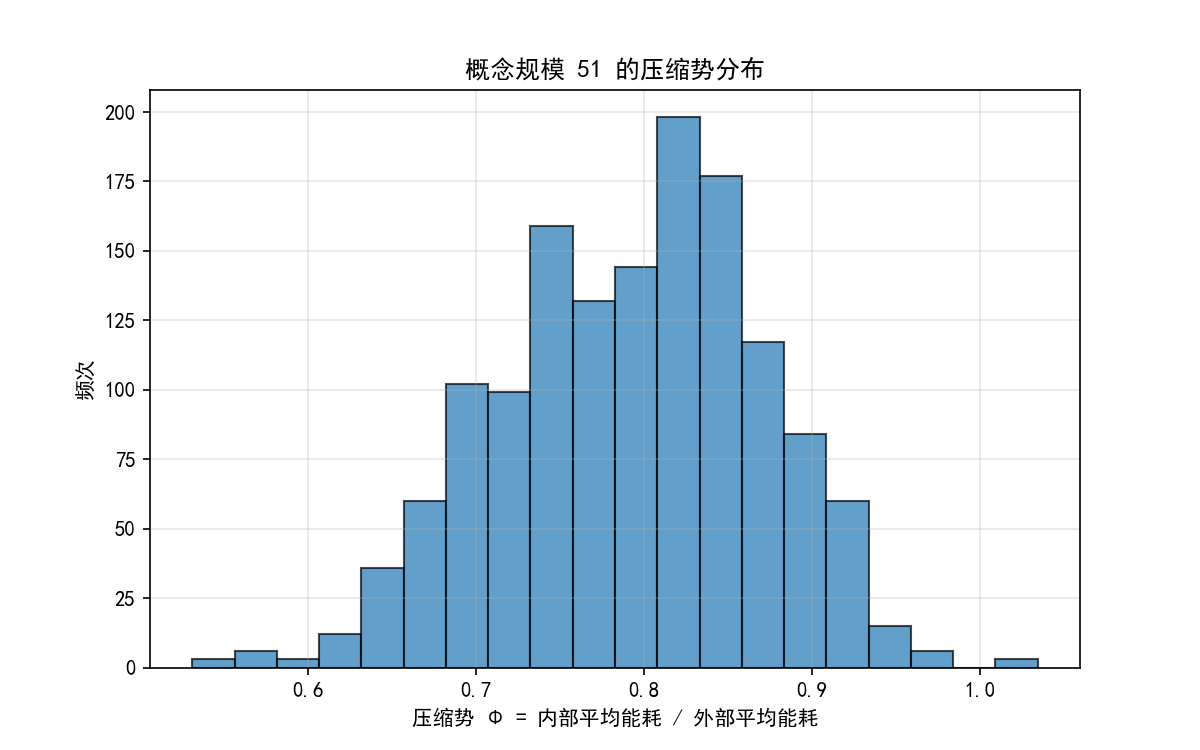
\includegraphics[width=\textwidth]{potential_dist_scale51.png}
    \caption{51 concepts ($\mu=0.793$, $\sigma=0.078$)}
    \label{fig:pot_51}
\end{subfigure}
\hfill
\begin{subfigure}[b]{0.45\textwidth}
    \centering
    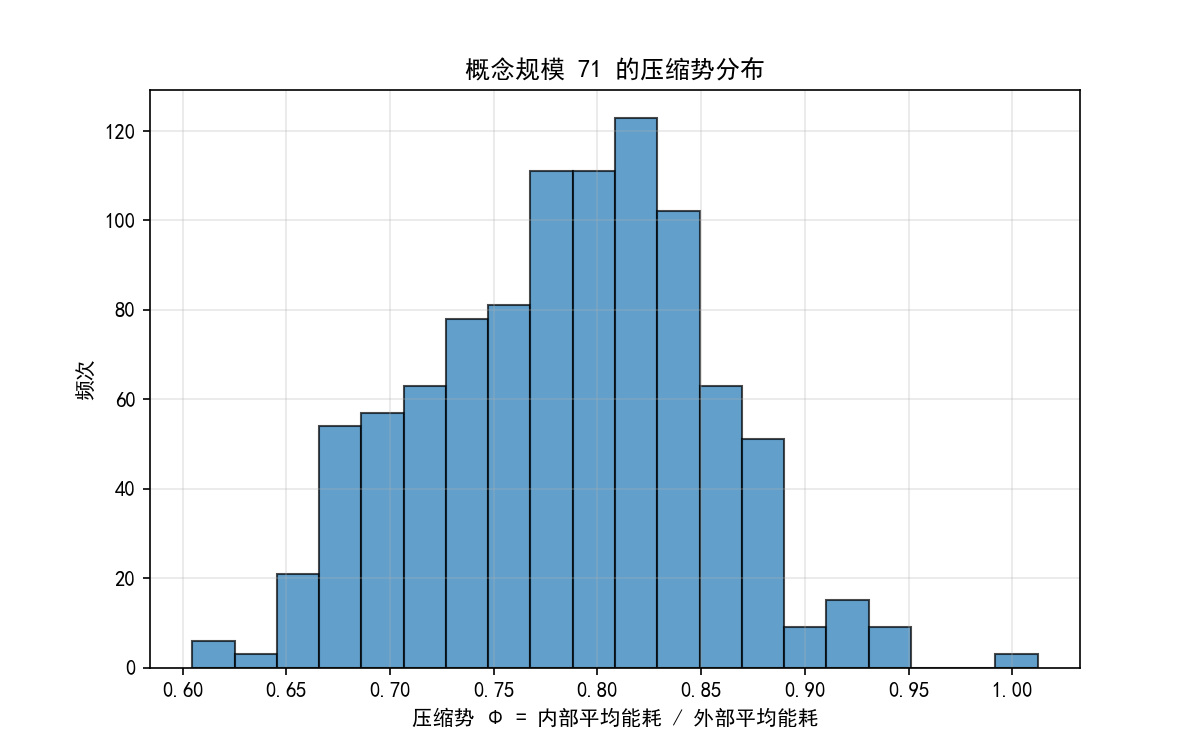
\includegraphics[width=\textwidth]{potential_dist_scale71.png}
    \caption{71 concepts ($\mu=0.784$, $\sigma=0.066$)}
    \label{fig:pot_71}
\end{subfigure}

\vspace{0.5cm}
\begin{subfigure}[b]{0.45\textwidth}
    \centering
    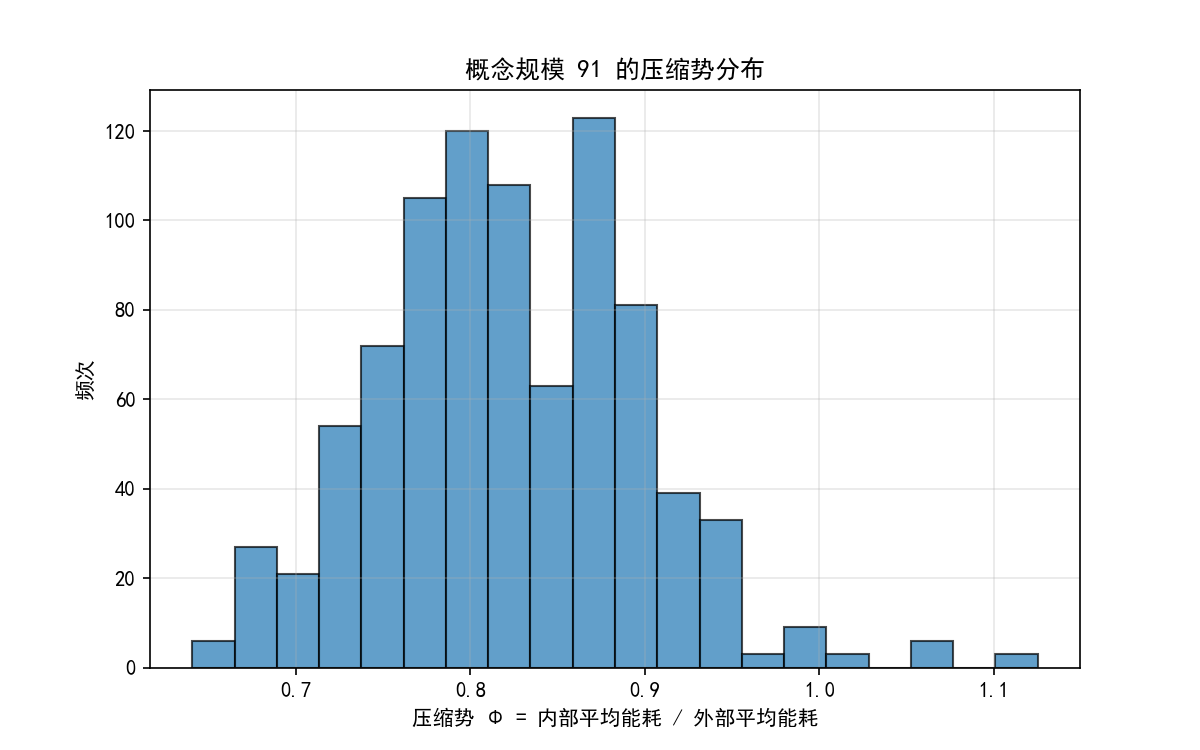
\includegraphics[width=\textwidth]{potential_dist_scale91.png}
    \caption{91 concepts ($\mu=0.822$, $\sigma=0.075$)}
    \label{fig:pot_91}
\end{subfigure}
\hfill
\begin{subfigure}[b]{0.45\textwidth}
    \centering
    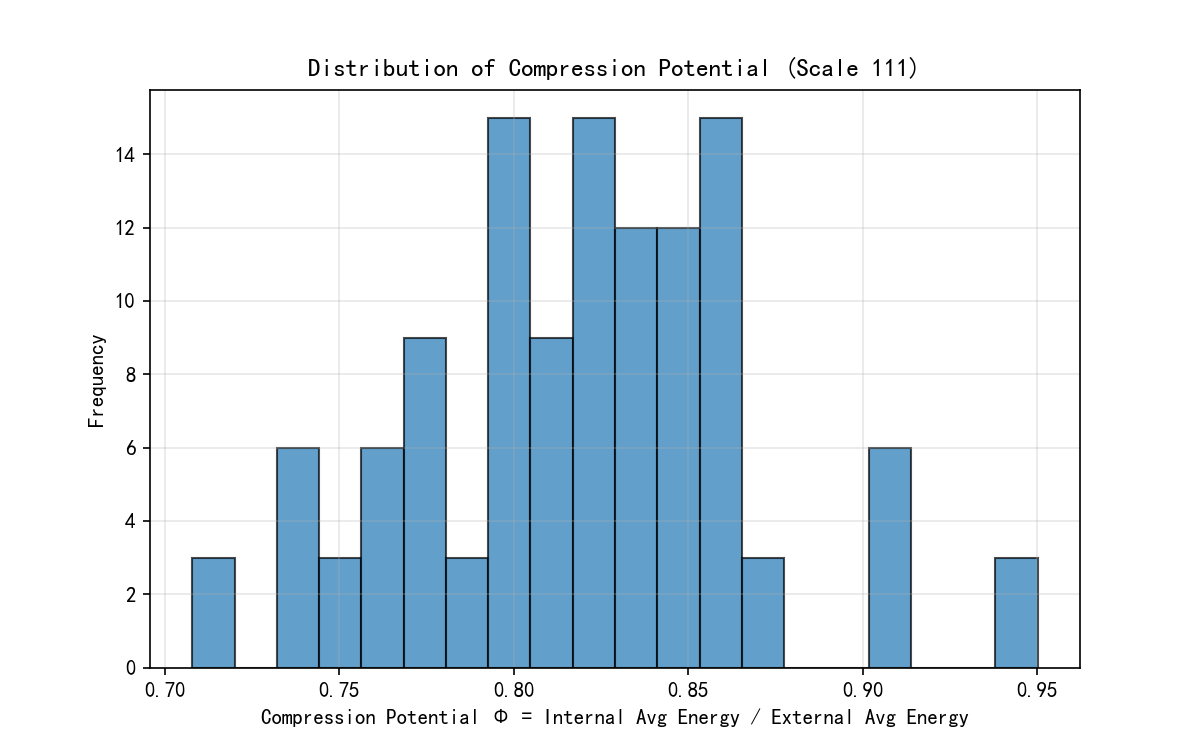
\includegraphics[width=\textwidth]{potential_dist_scale111.png}
    \caption{111 concepts ($\mu=0.820$, $\sigma=0.048$)}
    \label{fig:pot_111}
\end{subfigure}
\caption{Histogram of the compression potential $\Phi = E_{\text{internal}} / \bar{E}_{\text{external}}$ for all compression events across the four scales. The vertical axis represents frequency, and the horizontal axis represents the value of the compression potential. As the scale increases, the distribution of the compression potential becomes more concentrated (the standard deviation decreases from 0.078 to 0.048), while the mean remains stable around 0.8, indicating that the system shifts from extensive exploration to precise integration, and the energy characteristics of “good compression” remain consistent.}
\label{fig:potential_distribution}
\end{figure}

\begin{table}[h]
\centering
\caption{Summary of compression potential statistics (combined across three instances)}
\label{tab:potential_stats}
\begin{tabular}{lcccc}
\toprule
\textbf{Scale} & \textbf{Average Compression Potential $\bar{\Phi}$} & \textbf{Standard Deviation} & \textbf{Minimum} & \textbf{Maximum} \\
\midrule
51 Concept & 0.793 & 0.078 & 0.51 & 1.034 \\
71 Concept & 0.784 & 0.066 & 0.56 & 0.98 \\
91 Concept & 0.822 & 0.075 & 0.58 & 1.01 \\
111 Concept & 0.820 & 0.048 & 0.71 & 0.95 \\
\bottomrule
\end{tabular}
\end{table}

Observations reveal that although the number of compressions drops sharply from 1,416 (51 concepts) to 120 (111 concepts) as the scale increases, the mean compression potential remains stable between 0.78 and 0.82 (Table \ref{tab:potential_stats}). This stability suggests that, regardless of knowledge complexity, the system’s intrinsic criterion for “good compression” appears consistent—only clusters where internal energy consumption is approximately 80\% of external energy consumption are ultimately compressed. This provides quantitative evidence for energy minimization as a fundamental principle of cognitive organization.

Meanwhile, the standard deviation of the compression potential decreases with increasing scale (from 0.078 to 0.048), and the extremely low values ($\Phi < 0.6$) disappear entirely at 111 concepts. This is highly consistent with the observation in the main text that “compression density decreases while emergence intensity increases”: in low-complexity environments, the system extensively explores various possible clusters (of varying quality), whereas in high-complexity environments, the system selects only those clusters with clear energy advantages for precise integration, reflecting a strategic shift from “exploration” to “exploitation.”

Furthermore, the compression potential shows a positive correlation with the emergence intensity described in the main text (calculated comprehensively based on energy synergy, cohesion, etc.), though the compression potential reflects energy contrast more purely. The combination of these two indicators suggests that compressed clusters not only possess high energy synergy but also exhibit an internal-to-external energy consumption ratio consistent with energy-optimal expectations. This multi-faceted consistency further reinforces our understanding of conceptual compression as a natural byproduct of energy minimization.

\subsection{Emergent Patterns and Case Studies of Conceptual Compression and Principle Transfer}

\textbf{Scale dependence of concept compression.} In a 51-concept environment, the system extensively tested various concept combinations, such as the compression of “algorithm + neural network + machine learning + computer vision” (emergence strength 0.795), which exhibited high compression density but moderate emergence strength (0.79–0.84). As the scale increases, compression gradually focuses on semantically tight clusters: at 71 concepts, highly cohesive compressions such as “reinforcement learning + transfer learning + agents + generative adversarial networks + pattern recognition” emerge (emergence strength 0.825); with 91 concepts, a deep integration of “cognitive load + theory of mind + embodied cognition + cognitive neuroscience” emerges (emergence strength 0.819); and at 111 concepts, highly integrated principle-based clusters formed, such as “Operating Systems + Data Structures + Computer Networks + Software Engineering + Databases + Algorithms + Distributed Systems” (emergence intensity 0.967), reflecting a strategic shift from broad exploration to deep integration.

\textbf{Emergent characteristics of principle transfer.} A total of 7 instances of principle transfer were observed in the experiment, primarily concentrated in the 71/91 conceptual environment. Typical pathways included “Developmental Psychology → Pattern Recognition → Metacognition” (efficiency 0.371) and “Pattern Recognition → Generative Adversarial Networks → Agents” (efficiency 0.449). “Pattern Recognition,” as a core principle node, appeared in 6 of the 7 transfers, highlighting its status as a cognitive primity. In the 111-concept environment, only 1 transfer was retained (Developmental Psychology → Pattern Recognition → Metacognition), with an efficiency of 0.387, indicating that the system retains only the most reliable, validated paths in extremely complex environments. A detailed list of all transfer cases is provided in Appendix C.

By comparing representative compression and migration cases across different scales (Table \ref{tab:app_compression_cases}), we can clearly observe a continuous spectrum of system strategy evolution as knowledge complexity increases.

\subsection{Explanation of Deterministic Evolution}

The naturally emerging model constructed in this study exhibits deterministic evolution. Once the initial network and system parameters are fixed, subsequent evolution is driven by deterministic rules (with random exploration in soft perestroika controlled by a fixed seed), and the results of multiple runs are identical. Therefore, the results of a single run reported in this paper represent the deterministic behavior under that specific parameter configuration.

\subsection{Visualization of Experimental Results}

Figure \ref{fig:performance_comparison} shows a comparison of energy savings rates for the four models across four scales, while Figure \ref{fig:scale_effect} compares the scaling curves of the naturally emerging model and the preset algorithm model. Together, these two figures validate the advantages of the naturally emerging mechanism in terms of absolute performance and scaling robustness.

\begin{figure}[H]
\centering
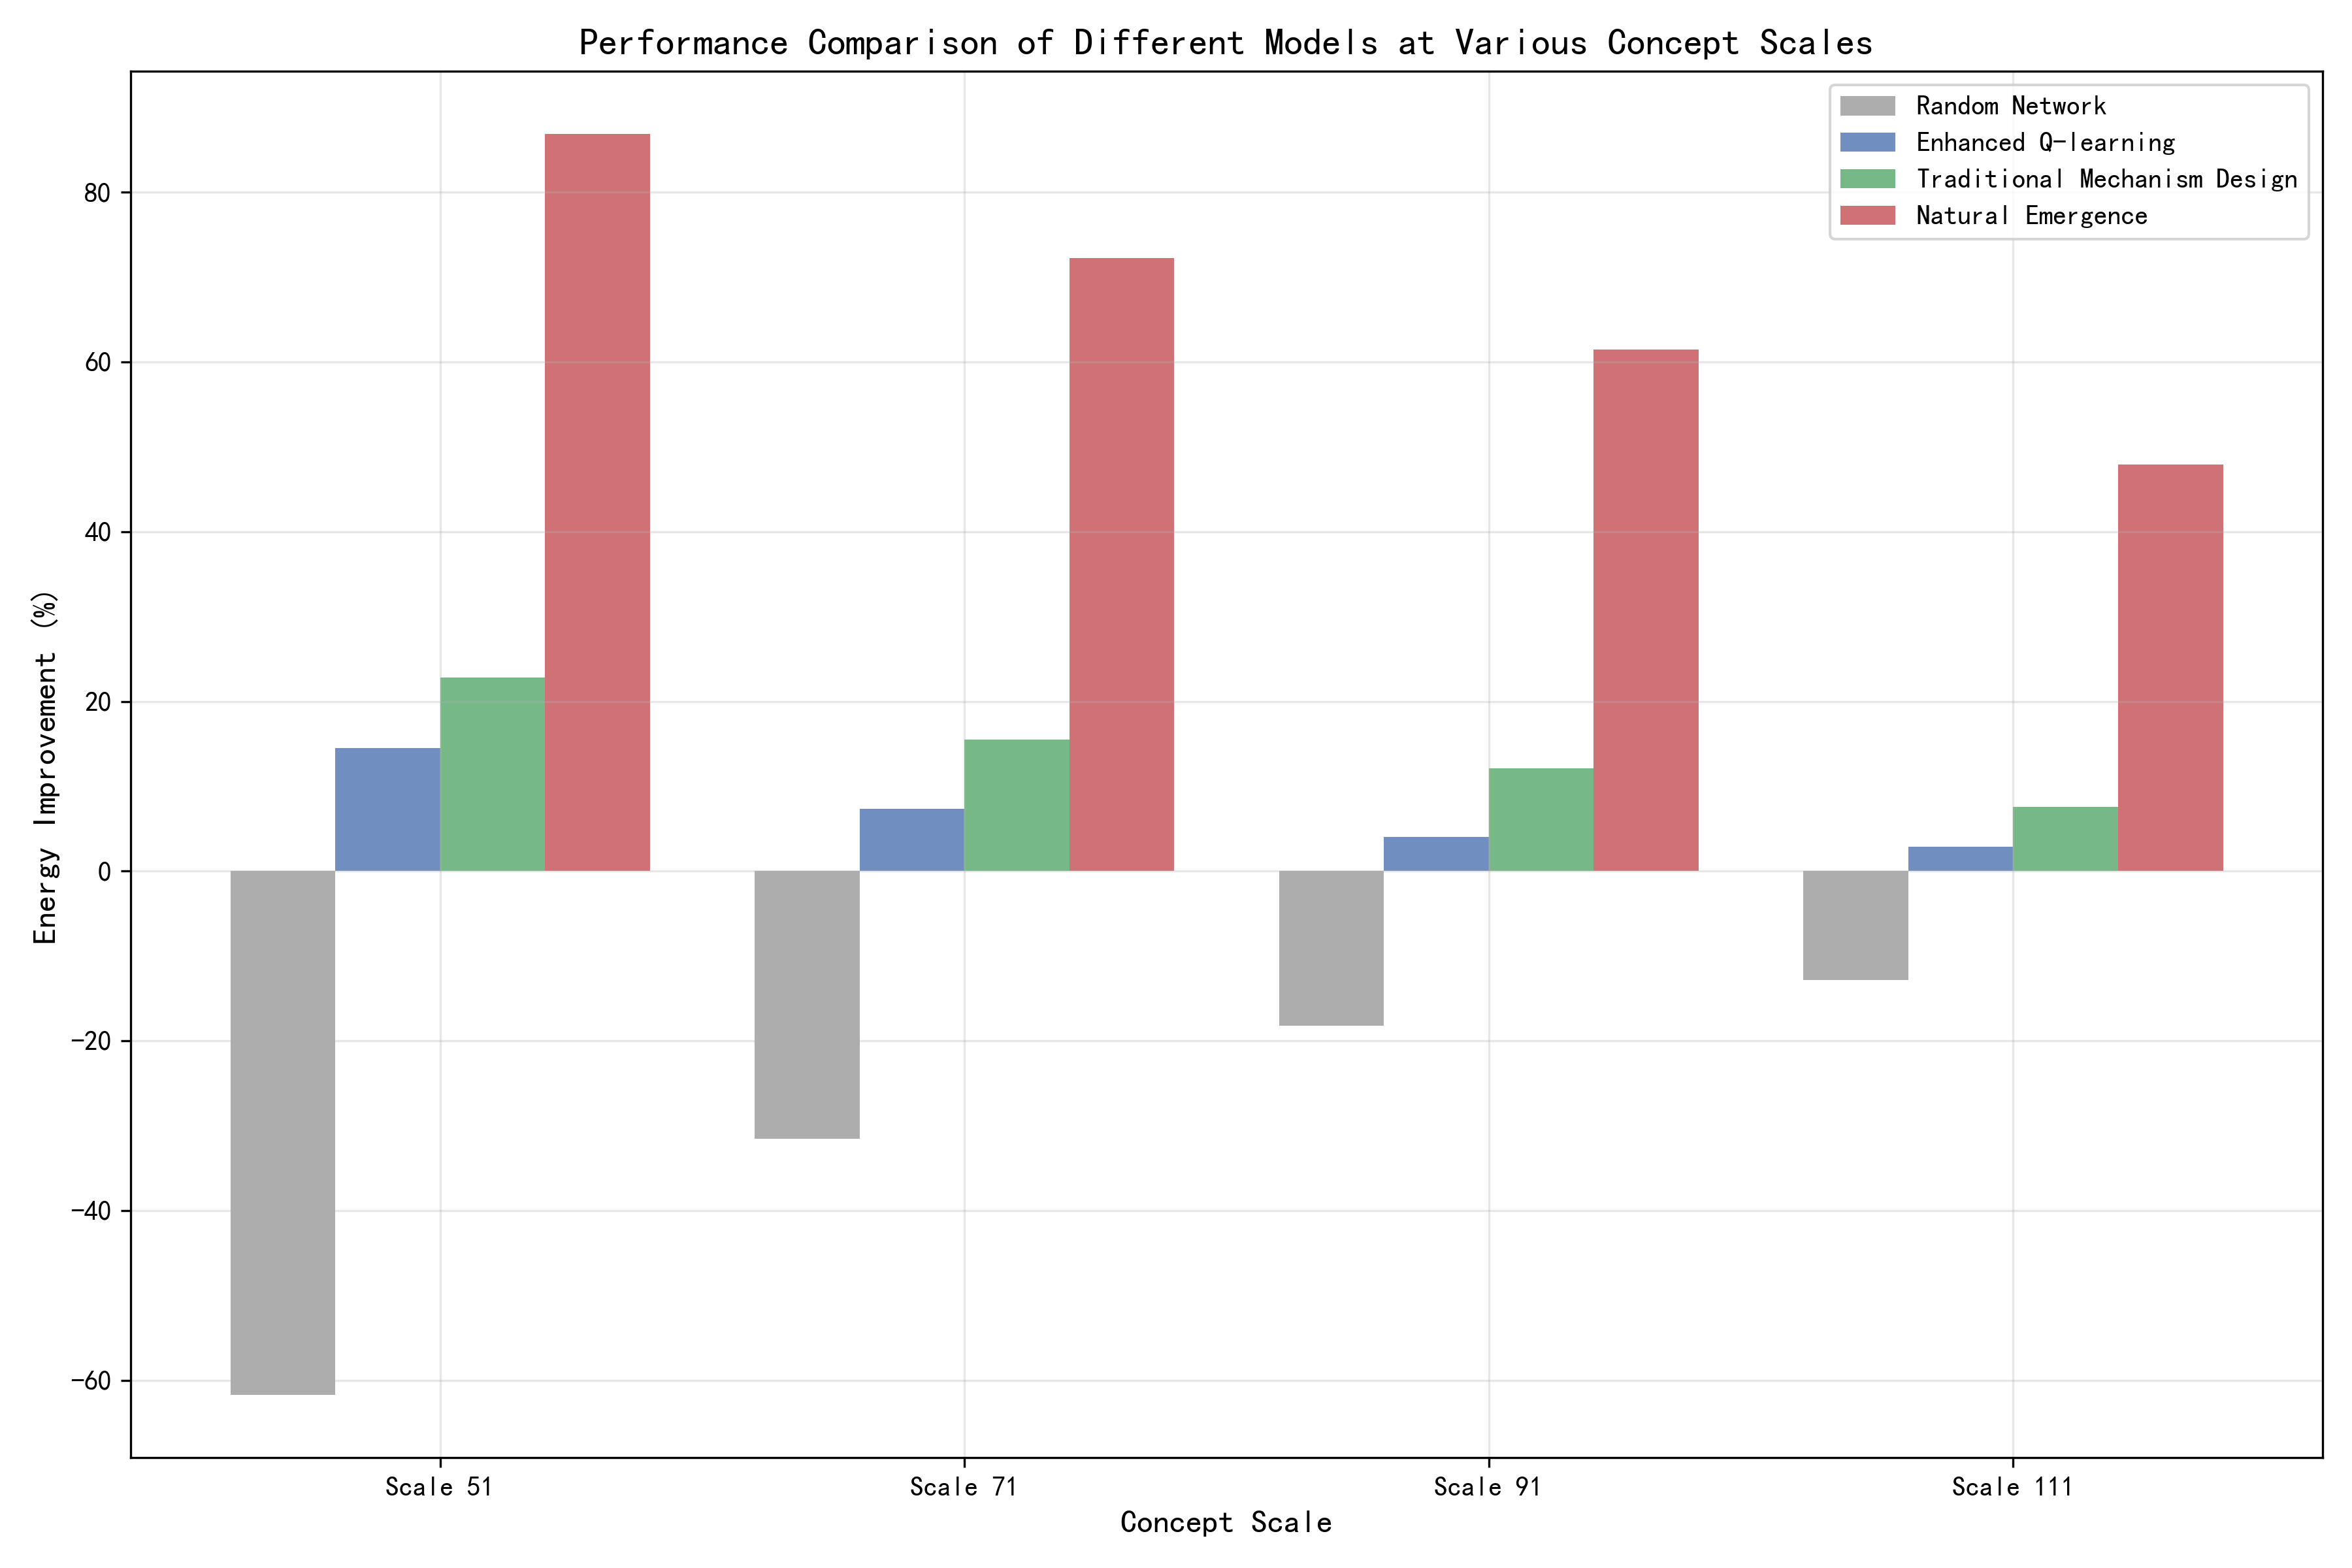
\includegraphics[width=0.85\textwidth]{fig6_performance.png}
\caption{Performance comparison of four models: Energy improvement rates of random network, Q-learning, preset algorithm, and naturally emerging models at scales of 51, 71, 91, and 111 concepts. The naturally emerging model significantly outperforms the other models at all scales, especially achieving an 86.9\% energy reduction at 51 concepts, demonstrating the strong driving force of energy minimization as a cognitive organization principle.}
\label{fig:performance_comparison}
\end{figure}

\begin{figure}[H]
\centering
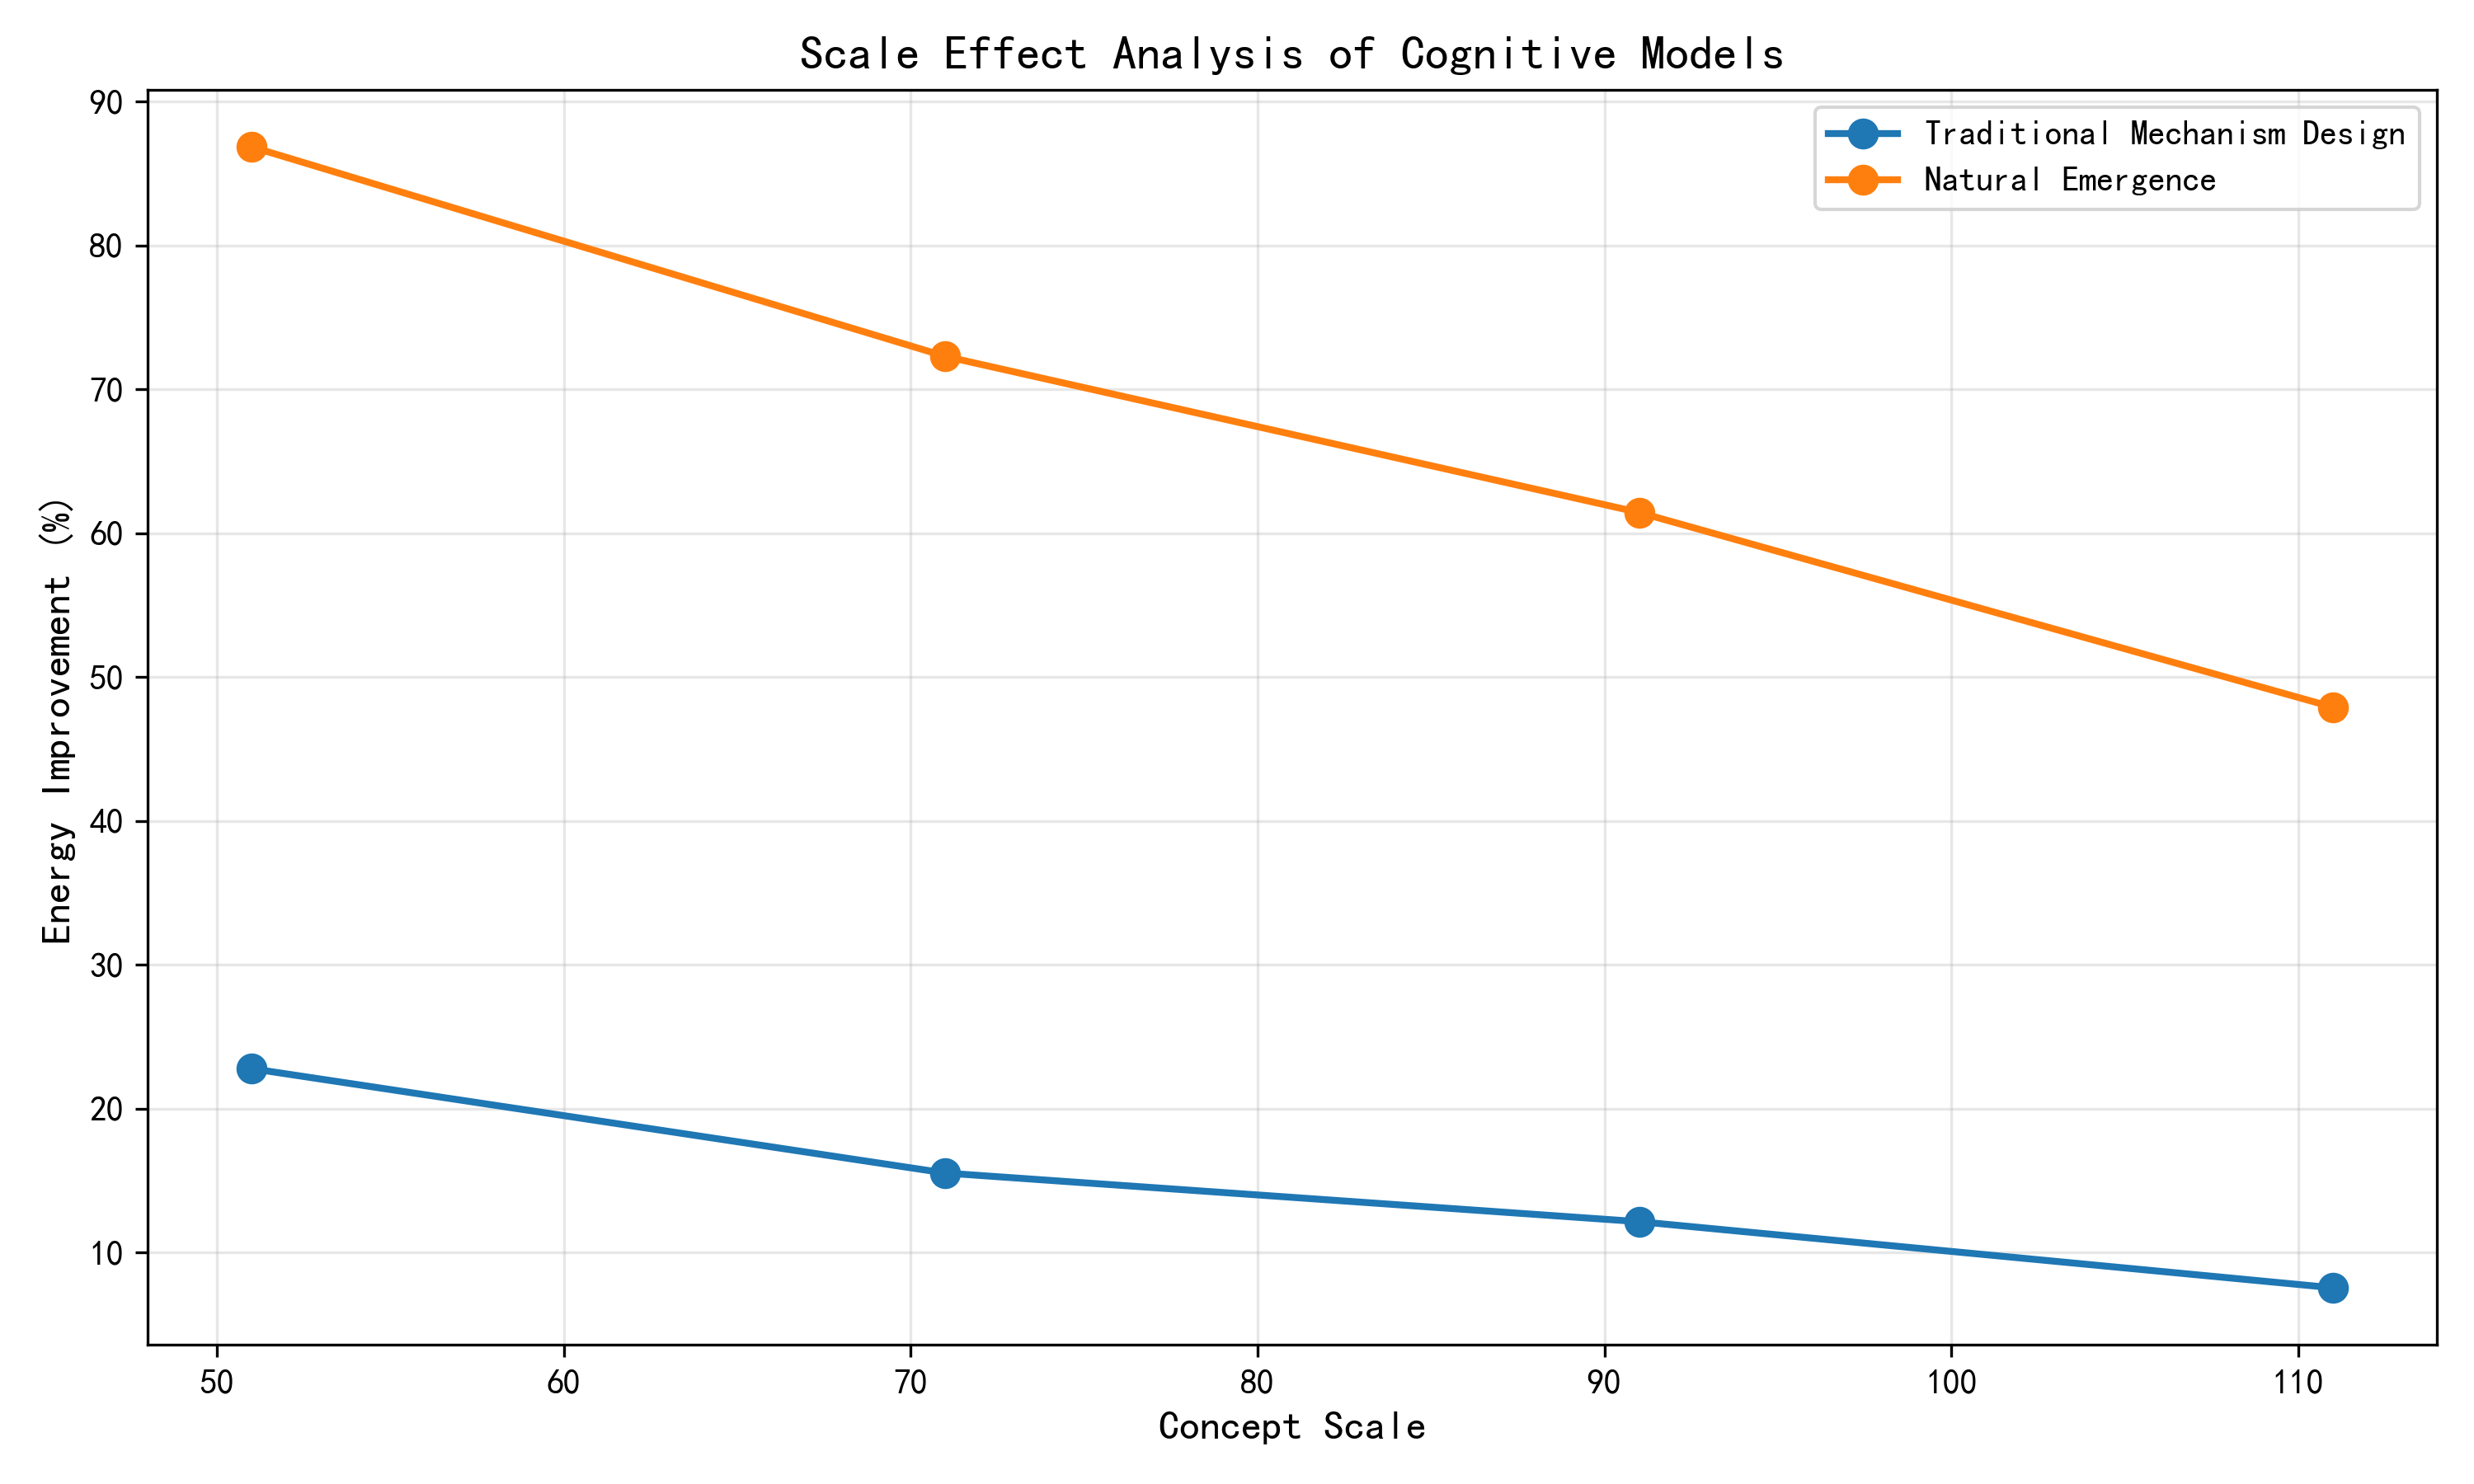
\includegraphics[width=0.95\textwidth]{fig7_scale_effect.png}
\caption{Scale effect curves: Trends in energy improvement rates of the preset algorithm model and the naturally emerging model as the number of concepts increases.}
\label{fig:scale_effect}
\end{figure}

Detailed comparison data (including comparisons with random networks and Q-learning), cognitive state distributions, and lists of all compression and migration cases are provided in Appendix C.

\subsection{Sensitivity analysis of the compression threshold}
\label{sec:threshold_sensitivity}

Section 7.3 uses a unified compression synergy threshold $\theta_c = 0.76$ for emergence detection. To examine the impact of this choice of observation parameter on the results, we take a concept scale of 91 as an example, scan $\theta_c$ from 0.5 to 0.9 in 0.05 increments, and record the number of compression events detected at each threshold. The results are shown in Table \ref{tab:threshold_scan}.

\begin{table}[H]
\centering
\caption{Number of detected compressions under different compression coherence thresholds (91 concepts, 10,000 iterations)}
\label{tab:threshold_scan}
\begin{tabular}{lccccccccc}
\toprule
Threshold $\theta_c$ & 0.50 & 0.55 & 0.60 & 0.65 & 0.70 & 0.75 & 0.80 & 0.85 & 0.90 \\
\midrule
Number of compressions & 301 & 301 & 301 & 295 & 271 & 259 & 101 & 0 & 0 \\
\bottomrule
\end{tabular}
\end{table}

The following patterns can be observed in the table:
\begin{itemize}
    \item When $\theta_c \leq 0.6$, the number of compressions stabilizes at 301, indicating that the compression clusters generated by the system generally exhibit internal coherence higher than 0.6; these clusters are robust products driven by energy dynamics.
    \item In the interval $0.65 \leq \theta_c \leq 0.75$, the number of compressions decreases slowly but remains above 250, suggesting that the emergence intensity of most compression clusters falls within this range.
    \item When $\theta_c$ rises to 0.8, the number of compressions drops sharply to 101, a decrease of 61\%; while for $\theta_c \geq 0.85$, no compression events are detected. This phenomenon reveals that there is a natural upper bound for the emergence intensity of compression clusters (around 0.8), and clusters exceeding this threshold are extremely rare in the system.
\end{itemize}

The above results imply the following:
\begin{enumerate}
    \item \textbf{Robustness of the phenomenon}: Within the broad threshold range of 0.5 to 0.75, the number of compressions remains at a high level, indicating that conceptual compression is a robust emergent feature in system evolution, rather than an artifact dependent on the arbitrary setting of a specific threshold.
    \item \textbf{Rationality of Threshold Selection}: The value of $\theta_c = 0.76$ used in the original experiment lies at the beginning of the declining region. This value captures the vast majority of compression events (259 instances) while avoiding the misinterpretation of background fluctuations in energy dynamics as emergent phenomena due to an excessively low threshold; it is a reasonable observation point that balances sensitivity and specificity.
    \item \textbf{Potential connection to phase transition theory}: The interval of steep decline in the number of compressions ($0.75 \to 0.80$) corresponds to the vicinity of the cognitive phase transition threshold observed in Section 6.5. This suggests that the distribution of the compression potential may be related to the system’s critical behavior, providing a clue for further exploration of the microscopic basis of cognitive phase transitions.
\end{enumerate}

This sensitivity analysis indicates that the compression phenomenon persists stably within a broad threshold range of 0.5 to 0.75. For thought experiments, the “optimality” of parameter selection is not the core issue; rather, the key lies in the robustness of the phenomenon—as long as a reasonable parameter range is specified, the system can spontaneously generate statistically regular compression and migration behaviors, which is sufficient to validate the validity of the axioms. This analysis aims to address concerns regarding the subjectivity of parameter selection and provides a reference for selecting appropriate thresholds when applying this framework to different fields of knowledge in future research.

\subsection{Universal Laws of Energy Evolution: Power-Law Decay}

In addition to qualitative observations of emergent phenomena, we conducted a quantitative analysis of the macroscopic dynamics of system evolution. In experiments conducted at four scales (51, 71, 91, and 111 concepts), the trajectory of global cognitive energy consumption $E(t)$ as the number of iterations decreases could be described by the power-law function $E(t) = a t^{-b} + c$ (with a goodness-of-fit $R^2$ close to 1.0). Table \ref{tab:energy_decay_fit} summarizes the fit metrics and emergence statistics averaged across scales.

\begin{table}[H]
\small
\centering
\caption{Fitting results for energy decay curves and emergence statistics across different scales (averaged across three individuals)}
\label{tab:energy_decay_fit}
\begin{tabular}{lccccc}
\toprule
\textbf{Scale} & \textbf{EEIR (\%)} & \textbf{$R^2$} & \textbf{RMSE} & \textbf{Total Comp.} & \textbf{Total Trans.} \\
\midrule
51 & 87.9 & 1.0 & 0.003 & 471.3 & 0.0 \\
71 & 75.7 & 1.0 & 0.002 & 317.3 & 3.0 \\
91 & 63.9 & 1.0 & 0.002 & 301.3 & 2.0 \\
111& 45.6 & 1.0 & 0.001 & 35.3 & 0.0 \\
\bottomrule
\end{tabular}
\end{table}

In the table, $R^2$ all reach 1.0 and RMSE is extremely low (0.001–0.003), indicating that energy consumption evolution exhibits a high degree of regularity rather than random fluctuations in the thought experiment environment under consideration. This form of power-law decay bears an interesting analogy to relaxation processes in physical systems, suggesting that cognitive dynamics driven by the energy minimization postulate may follow some universal scaling behavior. As the conceptual scale increases, the power exponent $b$ monotonically decreases (from approximately 0.32 for 51 concepts to 0.18 for 111 concepts), reflecting the moderating effect of knowledge complexity on the rate of energy decay; however, the fundamental power-law form is maintained across different levels of complexity. Figure \ref{fig:energy_decay_example} shows the energy consumption decline curve for a single individual at a concept scale of 51 and its fit; it can be seen that the actual evolutionary trajectory closely aligns with the power-law function.

\begin{figure}[H]
\centering
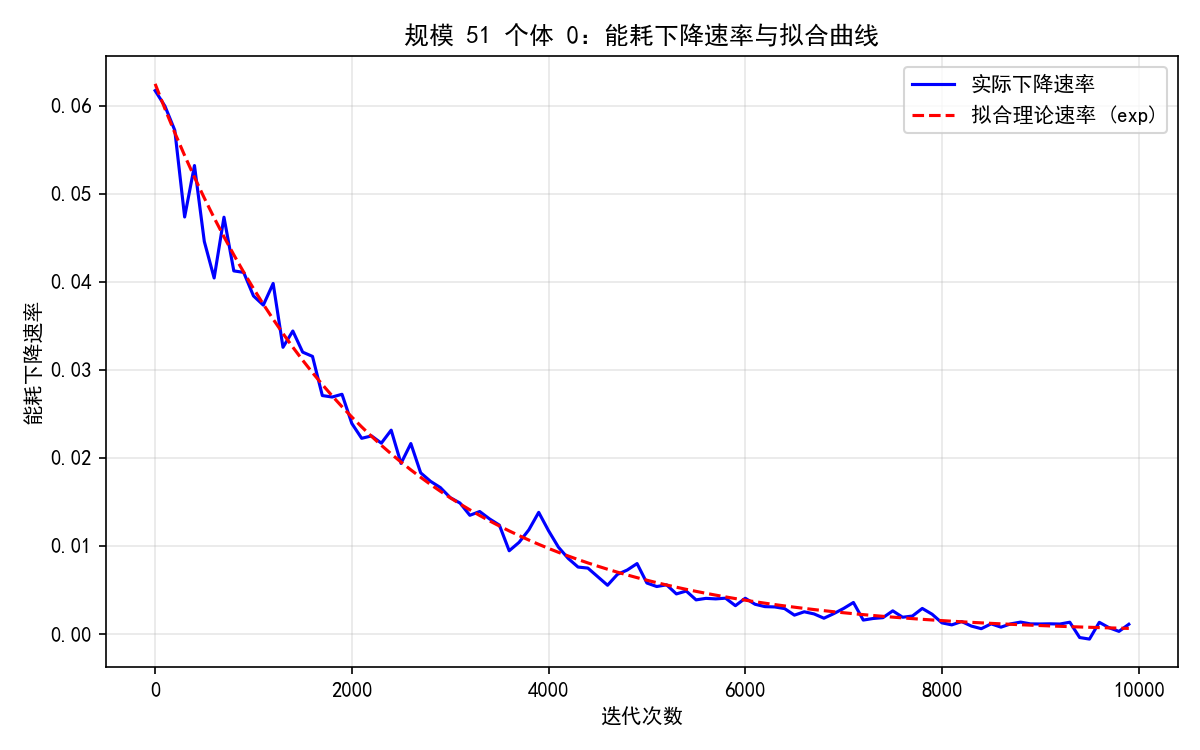
\includegraphics[width=0.7\textwidth]{energy_rate_scale51_ind0.png}
\caption{Evolution of cognitive energy consumption as a function of the number of iterations for a system of 51 concepts (individual 0). X-axis: Number of iterations (0–10,000). Y-axis: Global cognitive energy consumption $E(t)$. The blue solid line represents the system’s actual evolution trajectory, while the red dashed line represents the least-squares fit of the power-law function $E(t)=a t^{-b}+c$. The goodness-of-fit $R^2=1.0$ and root-mean-square error RMSE $=0.003$ indicate that the decline in energy consumption follows a highly deterministic power-law decay pattern. This curve represents the typical behavior of the three individuals at this scale; curves for other scales (71, 91, and 111 concepts) exhibit similar shapes but differ in decay rates (see Table \ref{tab:energy_decay_fit}).}
\label{fig:energy_decay_example}
\end{figure}

This observation provides support at the macroscopic dynamical level for energy minimization as a first principle of cognitive organization: the system not only reaches a low-energy state at its endpoint, but its entire evolutionary path also exhibits a simple mathematical law, which remains stable across different levels of knowledge complexity.

\subsection{Analysis of Computational Efficiency: Low-Energy, Low-Cost Natural Emergence}

To address the potential question of whether “cognitive graph theory is merely a computationally expensive toy,” we further measured the system’s actual runtime. All experiments were conducted on a standard laptop (Intel i7, 16GB RAM, no GPU acceleration) using a pure Python implementation. Table \ref{tab:time_comparison} compares the average runtime for core evolution (without any observation) versus full evolution (including compression/migration detection) across four scales.

\begin{table}[H]
\centering
\caption{Average runtime for core evolution and full evolution (seconds, 10,000 iterations, average of 3 runs)}
\label{tab:time_comparison}
\begin{tabular}{lccc}
\toprule
\textbf{Scale} & \textbf{Core Evolution (No Detection)} & \textbf{Full Evolution (with Detection)} & \textbf{Time Ratio} \\
\midrule
51 Concepts & 2.19 & 5.80 & 2.65x \\
71 Concept & 3.25 & 8.58 & 2.64x \\
91 Concept & 4.51 & 11.86 & 2.63x \\
111 Concept & 7.19 & 18.28 & 2.54x \\
\bottomrule
\end{tabular}
\end{table}

Even for the most complex 111-node conceptual network, a full evolution requiring 10,000 iterations (covering thousands of compression/transition detections) takes only about 18 seconds. The core evolution (i.e., pure energy dynamics) takes only about 7 seconds. This computational overhead is far lower than that of any deep learning-based model—the latter often requires thousands of GPU hours for training, and a single forward inference may consume milliwatt-level power. Our model runs on a standard laptop, and its energy consumption is negligible.

This extreme computational efficiency stems from two fundamental reasons: first, the system’s evolution relies solely on local energy updates, without backpropagation or global optimization; second, we deliberately avoided any “large” datasets—the system requires no pre-training, and all knowledge derives from the definition of the initial semantic network. This indirectly confirms the inherent energy-efficiency advantages of “principle-driven” models, standing in stark contrast to the current AI field’s reliance on massive computational power.

This result also echoes the argument in Section 8.2: principle-based cognitive models have the potential to bypass brute-force computation and achieve the emergence of higher-order cognitive functions with extremely low energy consumption.

\subsection{Power-Law Distribution of Concept Occurrence Frequency: Scale-Free Characteristics of Cognitive Systems}

To further explore the intrinsic organizational patterns of cognitive structures driven by energy minimization, we statistically analyzed the occurrence frequencies of concepts across all naturally emerging compression events. We examined two metrics: (1) the number of times a central node appears—the number of times each concept served as a compression center; (2) total node occurrence—the total number of times each concept (whether as a center or a member) appears. After sorting the frequencies in descending order, we performed linear regression on a double-logarithmic scale, with the results shown in Figure \ref{fig:zipf_distributions}.

\begin{figure}[H]
\centering
\begin{subfigure}[b]{0.45\textwidth}
    \centering
    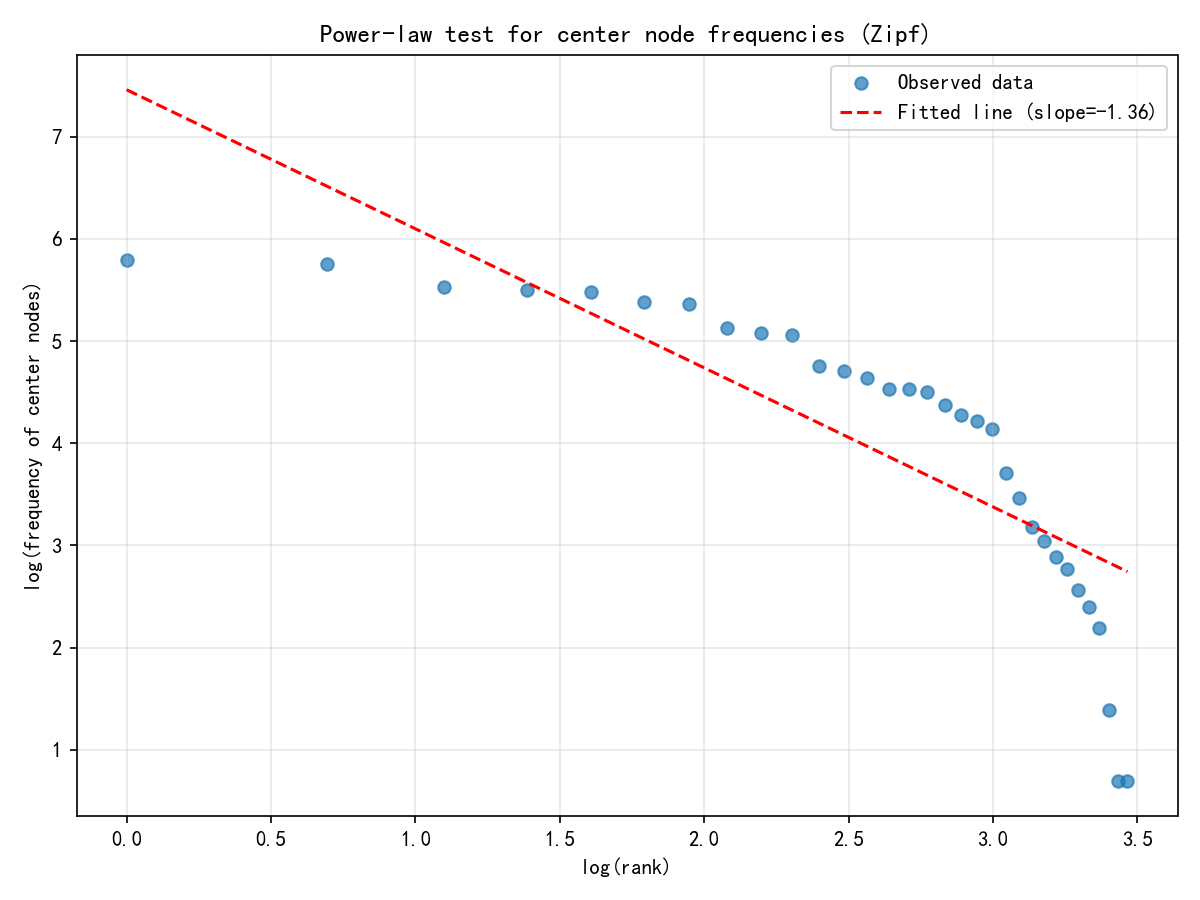
\includegraphics[width=\textwidth]{zipf_center.png}
    \caption{Central node occurrences}
    \label{fig:zipf_center}
\end{subfigure}
\hfill
\begin{subfigure}[b]{0.45\textwidth}
    \centering
    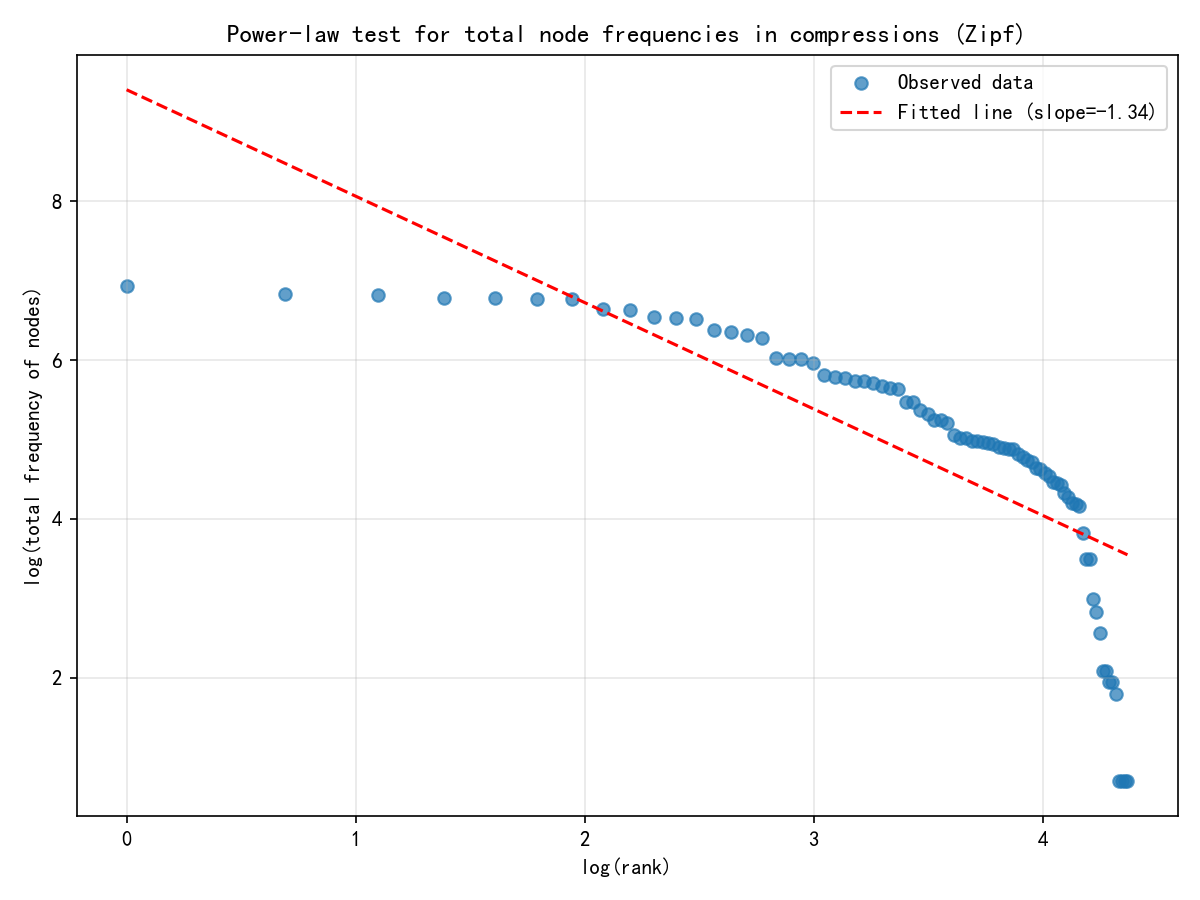
\includegraphics[width=\textwidth]{zipf_node_total.png}
    \caption{Total node occurrences}
    \label{fig:zipf_total}
\end{subfigure}
\caption{Double-logarithmic distributions of concept occurrence frequencies in compression events and their power-law fits. X-axis: rank $r$ sorted by frequency (log scale), Y-axis: frequency $f(r)$ (log scale). Scatter points are actual observations, straight lines are least-squares linear fits (i.e., power-law $f(r)\propto r^{-\alpha}$). (a) Central node occurrences: frequency of 32 distinct central nodes across 3376 compression events, power-law exponent $\alpha=-1.360$, goodness of fit $R^2=0.654$, $p=2.1\times10^{-8}$. (b) Total node occurrences: frequency of 79 distinct nodes across 21469 total appearances, power-law exponent $\alpha=-1.341$, $R^2=0.602$, $p=4.6\times10^{-17}$. Both distributions show that a few core concepts (e.g., “Algorithm,” “Operating System”) dominate the compression process, reflecting the scale-free structure spontaneously formed by cognitive networks driven by energy minimization, which is highly similar to Zipf’s law in natural language.}
\label{fig:zipf_distributions}
\end{figure}

Both distributions exhibit characteristics consistent with a power law, with key statistics summarized in Table \ref{tab:zipf_stats}.

\begin{table}[H]
\small
\centering
\caption{Power-law fit results for concept occurrence frequencies}
\label{tab:zipf_stats}
\begin{tabular}{lcccc}
\toprule
\textbf{Metric} & \textbf{Exponent (slope)} & \textbf{$R^2$} & \textbf{$p$-value} & \textbf{Total Events} \\
\midrule
Central Node Occurrences & $-1.360$ & 0.654 & $2.1\times10^{-8}$ & 3376 \\
Total Node Occurrences & $-1.341$ & 0.602 & $4.6\times10^{-17}$ & 21469 \\
\bottomrule
\end{tabular}
\end{table}

The distribution of central node occurrences (3376 compression events, 32 distinct centers) reveals an important phenomenon: a few concepts (e.g., “Algorithm,” “Operating System,” “Relativity”) are repeatedly selected as compression centers, while most concepts rarely serve as centers. The distribution of total node occurrences (21,469 appearances, 79 distinct nodes) depicts the imbalance in the overall activity of concepts in compression events—abstract concepts with high generality frequently participate in compression, while concrete domain-specific concepts are less involved. This distribution pattern is an external manifestation of the “rich-get-richer” phenomenon typical in complex systems.

These distribution characteristics are highly consistent with scale-free networks in complex systems \citep{newman2005power}, and their statistical pattern (power exponent around $-1$) shows an interesting correspondence with the classic Zipf’s law \citep{zipf1949human}. In the cognitive domain, learning curves also often exhibit power-law forms \citep{anderson2001power}, providing a new observational perspective for linking this model to human cognitive patterns. Importantly, these statistical regularities are not produced by externally preset rules but are the result of the system’s spontaneous evolution driven by energy minimization. They provide new observational evidence for the model’s cognitive validity at the level of structural organization: in the pursuit of energy optimization, cognitive systems naturally evolve a core-periphery structure dominated by hub nodes and featuring sparse participation by most nodes. This bears a profound correspondence with the consolidation process of “core concepts” in human cognition and the statistical patterns of language use.

Furthermore, this distribution characteristic corroborates the phase transition behavior observed in Section 6.5—when the system crosses a critical point, a small number of principal nodes begin to dominate compression and migration, causing the macroscopic structure to exhibit scale-free features. This finding links energy dynamics with complex systems theory, suggesting that energy minimization may be a deep-seated driving force behind the criticality of self-organization in cognitive complex systems.

\section{Discussion}

\subsection{Theoretical Implications and Observations}

Through four scale-dependent thought experiments, this study observed behavioral patterns of cognitive systems across environments of varying knowledge complexity, offering new perspectives for cognitive science and artificial intelligence theory from multiple dimensions.

\textbf{Observations on scale-adaptive patterns}: As the number of concepts increased from 51 to 111, energy consumption optimization in the naturally emerging model decreased from 86.9\% to 47.9\% (a 45.6\% reduction), while in the pre-set algorithm model, it decreased from 22.8\% to 7.6\% (a 67.1\% reduction). This indicates that increased knowledge complexity poses a challenge to any cognitive system, but self-organizing mechanisms based on energy minimization are better equipped to address this challenge. In the 111-concept environment, the system shifted from extensive exploratory compression (51 concepts: 466 instances) to precise, principle-based integration (111 concepts: 43 instances), with compression density decreasing from 9.14 instances per concept to 0.39 instances per concept, reflecting a strategic shift from broad exploration to precise integration.

\textbf{The universality of energy optimization as an organizing principle}: Across different conceptual scales, energy minimization consistently emerges as an effective driving force for cognitive organization. The naturally emerging model achieved energy optimization rates of 86.9\%, 72.3\%, 61.4\%, and 47.9\% across the four scales, respectively, significantly outperforming the predefined algorithmic model. More importantly, the scale-dependent decay rate of the emerging model (45.6\%) is far smaller than that of the preset algorithm model (67.1\%) and the Q-learning model (78.5\%), suggesting that natural evolutionary mechanisms based on energy minimization possess better adaptability when handling increasing cognitive complexity.

\textbf{Emergent Characteristics of Creative Thinking Patterns}: Experiments observed that certain features of creative thinking manifest in distinct ways: in low-complexity environments, conceptual connections are extensively established but transfer has not yet formed (accumulation stage); in medium-complexity environments, cross-domain transfer begins to emerge (exploration stage); and in high-complexity environments, transfer is extremely cautious and highly precise (consolidation stage). These patterns show an interesting correspondence with Wallas’s four-stage theory of creative thinking, and the driving force remains energy minimization.

\textbf{Cognitive scale-free characteristics revealed by power-law distributions.} In addition to macroscopic energy evolution, the system’s microstructure also exhibits profound statistical regularities. We analyzed the frequency of concept occurrence across all naturally emerging compression events and found that both the number of appearances by central nodes and the total number of node appearances exhibit power-law distributions (Figure \ref{fig:zipf_distributions}, Table \ref{tab:zipf_stats}). This distribution pattern—where “a few hub nodes are frequently used while the majority of nodes participate sparsely”—is a hallmark of the self-organizing criticality and scale-free network structure characteristic of complex systems. In natural language, word frequency also follows a Zipf distribution \citep{zipf1949human}, and the frequency distribution of concepts in this model bears a striking resemblance to it. This provides an intriguing window into how energy-minimization-driven cognitive evolution spontaneously generates statistical patterns analogous to those found in human language use. This finding offers independent observational evidence, distinct from energy consumption metrics, for the cognitive rationality of the model: the system not only achieves optimization at the energy level, but its structural organization also exhibits statistical consistency with real cognitive systems (such as semantic networks). The presence of power-law distributions also corroborates the phase transition behavior observed in Section 6.5—when the system crosses the critical point, a small number of principal nodes begin to dominate compression and migration, causing the macroscopic structure to exhibit scale-free characteristics. The energy minimization principle thus links cognitive dynamics with complex systems theory, suggesting that it may be a deep-seated driving force behind the self-organizing criticality of cognitive complex systems.

\subsection{Implications for the Next Generation of AI Paradigms}

Bowers et al. have criticized methodological issues in current comparative studies of AI and human cognition. The observations in this paper offer a potential solution to this criticism: shifting from a data-driven to a principle-driven approach, and from statistical correlations to structural understanding.

\textbf{From predefined architectures to natural evolution.} The performance of predefined algorithmic models dropped significantly to 7.6\% in the 111-concept environment, while the naturally emerging model still maintained a strong performance of 47.9\%, suggesting that architectures based on natural evolution are more scalable than preset algorithms. This observation challenges the design philosophy of current AI systems that rely on preset architectures and rules, hinting that we should consider moving towards self-organizing, adaptive system designs.

\textbf{From statistical correlations to principled understanding.} High-quality transfer in the experiments is based on abstract principles (such as “pattern recognition”) rather than superficial similarities, and the same transfer pathways recur across different scales. This suggests that next-generation AI may focus on principled understanding rather than merely statistical correlations, achieving more effective cross-domain transfer by identifying deep structural similarities.

\textbf{A dialogue with the current frontier of AI: From data-driven to principle-driven.} Recent academic reflections on AI development suggest that large models have approached the limits of human data, and that true intelligence should resemble an infant’s self-learning through perception and action. The naturally emerging model presented in this paper relies entirely on large-scale training data. Starting solely from two fundamental postulates—“cognitive spacetime” and “energy dynamics”—it spontaneously generates conceptual compression and principle transfer through the principle of energy minimization, realizing a prototype of generative learning rather than data fitting. Experimental results demonstrate the potential of this approach: in a complex cognitive environment comprising 111 concepts, the naturally emerging model still achieves a 47.9\% energy reduction, while the traditional preset algorithm only achieves 7.6\%. More importantly, this optimization is spontaneous and unsupervised, requiring no labeled data for specific tasks. The conceptual compression observed in experiments (such as the deep integration of “Operating Systems + Data Structures + Networks + Software Engineering”) and principle transfer (such as “Pattern Recognition” serving as a bridge across domains) reflect the system’s insight—not surface-level correlations, but deep principled understanding. This principle-based cognitive framework naturally supports infinite tasks because it establishes general cognitive capabilities rather than specific task skills.

\textbf{Adaptive management of cognitive load.} In the 111-concept environment, the system spontaneously reduced the compression density from 9.14 to 0.39 operations per concept, and reduced the number of transfers from multiple times to just once, demonstrating intelligent cognitive load management. This offers insights for designing scalable AI systems: if a system can automatically adjust its cognitive strategies based on task complexity, it may help avoid computational bottlenecks in complex environments.

\textbf{Explicit modeling of algebraic structures.} The group-theoretic description of cognitive operations provides a new mathematical foundation for AI. Cognitive models based on algebraic structures may offer new insights into the current interpretability dilemma of neural networks by providing a rigorous mathematical description of cognitive processes.

\subsection{Connections to Neuroscience}

Our theoretical framework forms intriguing correspondences with several cutting-edge discoveries in neuroscience. The principle of energy efficiency resonates with the human brain’s energy budget, where it accounts for only 2\% of body weight yet consumes 20\% of basal metabolic rate; the phenomenon of concept compression density decaying with scale mirrors the process of synaptic pruning during development; the modular organization of structures corresponds to the natural boundaries of functional modules in the brain; and dynamic simulations of neural plasticity map onto mechanisms such as long-term potentiation and long-term depression. These correspondences suggest that energy minimization may not only be an organizational principle at the cognitive level but also a universal principle of structural optimization at the neural level. The review by Carlson et al. \cite{carlson2025attending} demonstrates the application of cognitive science to real-world issues (such as climate change awareness), further highlighting the interdisciplinary value of cognitive research.

\subsection{Limitations and Future Work}

Although this study has yielded some observations regarding cognitive computational modeling, several limitations remain, which also point to directions for future research.

\textbf{Discrepancy between network scale and real-world cognition}: Even a 111-concept network remains limited in scale compared to the knowledge systems of human experts; concept nodes employ concise definitions, lacking the hierarchical structures and fuzziness found in real-world knowledge; the mapping of meta-structures exhibits a reductionist tendency, failing to fully capture the lateral connections and metaphorical tensions inherent in holistic thinking. Future work could integrate knowledge bases such as WordNet and ConceptNet to construct cognitive networks comprising thousands of concepts, introduce hierarchical representations and fuzzy semantics, and explore meta-structures based on Chinese character radicals to better align with holistic Chinese thinking.

\textbf{Insufficient precision in modeling individual differences}: Currently, individual differences are introduced solely through random initialization, lacking systematic modeling based on cognitive styles. In the future, parametric models of cognitive styles could be established using psychological scales to simulate the cognitive development continuum from children to experts. The “cognitive compression style” conceptual framework proposed by A. Jacobs \cite{jacobs2026cognitive} could provide theoretical support for modeling individual differences.

\textbf{Lack of integration of multimodal perception and motor skills}: Current models are entirely based on abstract concepts and lack an embodied foundation for perception and motor skills. In the future, multimodal neural networks could be integrated to enable embodied validation on robotic platforms.

\textbf{Insufficient breadth and depth of empirical validation}: Current validation is primarily based on computational metrics and has not been directly compared with human behavioral data or brain imaging data. However, it should be noted that the purpose of this study is not empirical fitting, but rather to provide a compatible “possible world.” Should future research aim to examine the correspondence between this model and actual cognition, psychological experiments could be designed to test the model’s predictions, or multivariate pattern analysis could be conducted by comparing the model’s outputs with brain activity data—though this exceeds the scope of this paper, which is intended as a thought experiment platform. Cognitive science holds broad application prospects; as demonstrated by Carlson et al. \cite{carlson2025attending} in their study on climate change awareness, cognitive theories can guide the resolution of real-world problems.

\textbf{Requirements for mathematical refinement of the theoretical framework}: The application of group theory remains at the conceptual level, and topological properties and dynamical systems theory have not been fully explored. Future work could deepen the description using Lie groups and Lie algebras, apply topological data analysis to investigate the topological features of the cognitive space, and use bifurcation theory to explain cognitive phase transition phenomena.

\textbf{Contextual Dynamism and Cross-Cultural Extension}: The current model is based on the assumption of a single static context. In the future, context evolution operators could be introduced to construct a “context-knowledge” co-evolutionary system. By comparing Chinese and English bilingual cognitive networks, the cross-cultural universality of cognitive graph theory can be tested, providing computational model support for cultural psychology.

\textbf{Further exploration and validation of concept frequency distributions.} Although we observe consistency between concept occurrence frequency and power-law distributions, the current analysis has several limitations: First, the concept set is limited in size (only 79 nodes out of 111 concepts participated in compression events) which may affect the stability of the distribution; this phenomenon could be replicated in large-scale networks comprising thousands of concepts in the future. Second, the discrepancy between the power-law exponent (around -1.36) and the classic linguistic Zipf exponent (-1 \citep{zipf1949human}) may stem from differences in semantic similarity calculation methods, compression threshold settings, or the granularity of concept definitions; the underlying causes require further investigation through parameter sensitivity analysis and cross-domain comparisons. Finally, this study has only verified consistency with the power-law distribution and has not yet conducted a rigorous comparison with other distributions (such as the exponential distribution or the log-normal distribution). In the future, more systematic statistical methods (such as the framework proposed by Clauset et al. \citep{clauset2009power}) should be introduced to investigate whether the power-law distribution is the optimal descriptive model for these distributions. Additionally, cross-cultural comparisons of concept frequencies (such as between Chinese and English cognitive networks) will also help test the universality of this distributional pattern.

\section{Conclusion}

Through a series of thought experiments, this paper observes the phenomenon of energy-optimization-driven cognitive organization within the framework of cognitive graph theory across environments of varying knowledge complexity. Based on four scale experiments involving 51, 71, 91, and 111 cross-domain concepts, we observed the following core phenomena:

\begin{enumerate}
    \item \textbf{Energy minimization as a fundamental principle of cognitive organization}: The naturally emerging model achieved energy optimization of 86.9\%, 72.3\%, 61.4\%, and 47.9\% respectively, whereas the pre-set algorithmic model achieved only 22.8\%, 15.5\%, 12.2\%, and 7.6\%. The significant difference between the two suggests that energy minimization is a more fundamental principle of cognitive organization, whose effectiveness remains robust as knowledge complexity increases.

    \item \textbf{Concept compression density adapts and decreases with scale}: The concept compression density spontaneously formed by the system decreases from 9.14 for 51 concepts to 0.39 for 111 concepts (a 95.7\% decrease). This trend shows an interesting parallel with the cognitive development process in humans, which progresses from broad exploration to precise integration, reflecting the system’s adaptive strategic adjustments when facing different levels of knowledge density—extensive exploration in low-density environments and deep integration in high-density environments.

    \item \textbf{Emergence Window and Stability of Principle Transfer}: The number of transfers peaked at moderate complexity (71/91 concepts, 3 times each), while for the 111 concepts, it drops to just 1 time; meanwhile, transfer efficiency remains stable between 0.35 and 0.45. “Pattern Recognition” served as the core principle node, appearing 6 times out of 7 migrations, highlighting the key role of abstract principles in cross-domain connections. The repeated emergence of the same migration path across different scales (e.g., developmental psychology → pattern recognition → metacognition) suggests that its effectiveness has been validated through environmental screening.

    \item \textbf{Critical phenomenon at the 111-concept threshold}: In the 111-concept environment, the system’s strategy undergoes a fundamental shift—concept compression plummeted from 301 to 43, with only 1 instance of principle migration. This suggests that under extreme complexity, the cognitive system triggers a strategic phase transition, shifting from “exploratory integration” to “conservative maintenance,” retaining only the most essential integrations and migrations.

    \item \textbf{The stability of the compression potential confirms the unified driving force of energy minimization}: although the number of concept compressions decreases with scale, the compression potential of compressed clusters remains stable at around 0.8, and the standard deviation decreases with scale. This indicates that the system maintains a consistent internal standard for “good compression” across different levels of complexity, shifting from broad exploration to precise integration.

    \item \textbf{The power-law distribution of concept occurrence frequencies reveals the scale-free characteristics of cognitive systems.} The distributions of central nodes and total node occurrences both exhibit high consistency with power-law distributions ($R^2>0.6$, $p<10^{-8}$), indicating that cognitive networks, driven by energy minimization, spontaneously evolve a core-periphery structure dominated by a few hub nodes and characterized by sparse participation of the majority of nodes. This statistical pattern bears a strong resemblance to Zipf’s law in natural language \citep{zipf1949human}, providing cross-domain observational evidence for the cognitive validity of the model that is independent of energy consumption metrics.
\end{enumerate}

These observations offer a new theoretical perspective for understanding the organization of human cognition: cognitive systems spontaneously form higher-order functions such as conceptual compression and principle transfer through the first-principle of energy minimization, and are capable of adaptively adjusting cognitive strategies based on knowledge complexity. This work also reveals the possibility of a paradigm shift in AI from “data-driven” to “principle-driven”—endowing machines with the intrinsic ability to perceive and optimize “cognitive energy consumption,” allowing AI to move from statistical correlation to structural understanding, and from mechanical execution to creative thinking. The cognitive graph theory framework based on energy optimization provides a preliminary theoretical foundation and exploration path for realizing this vision.

\newpage

\bibliography{references}

\newpage

\appendix

\section{Details of the Algebraic Framework Validation}
\label{app:algebraic_validation}

This appendix provides the detailed setup, data, and results of the algebraic framework validation experiments described in Section 5.

\subsection{Experimental Design}

\textbf{Experiment 1: Verification of Cognitive Operation Semigroups}
\begin{itemize}
    \item Objective: To observe whether basic cognitive operations (iteration, learning, forgetting, compression, and transfer) satisfy the properties of a semigroup under composition.
    \item Method: Randomly generate 13 cognitive operations and test the associative law: $(a \circ b) \circ c = a \circ (b \circ c)$.
\end{itemize}

\textbf{Experiment 2: Observation of Noetherian Correspondences}
\begin{itemize}
    \item Objective: To observe the correspondence between cognitive symmetries and conserved quantities.
    \item Method: Detect symmetries in cognitive networks with 5, 10, and 15 nodes, and calculate the relative changes in conserved quantities (global energy, structural entropy, fractal dimension).
\end{itemize}

\textbf{Experiment 3: Observation of the Applicability of the Orbit-Stabilizer Theorem}
\begin{itemize}
    \item Objective: To observe the manifestation of the Orbit-Stabilizer Theorem in the cognitive state space.
    \item Method: Calculate the size of the cognitive symmetry group $|\cognitivegroup|$, the size of the stabilizers $|\text{Stab}(G)|$, and the size of the orbits $|O_G|$, and verify $|O_G| = \frac{|\cognitivegroup|}{|\text{Stab}(G)|}$.
\end{itemize}

\textbf{Experiment 4: Demonstration of a Lie Group Evolution Framework}
\begin{itemize}
    \item Objective: To demonstrate the feasibility of describing continuous-time cognitive evolution using Lie groups.
    \item Method: Three different combinations of Lie algebra generators (energy optimization driven, concept compression-driven, and principle transfer-driven) were employed to observe changes in cognitive energy consumption before and after evolution.
\end{itemize}

\textbf{Experiment 5: Scalability Testing of the Algebraic Method}
\begin{itemize}
    \item Objective: To evaluate the computational efficiency of the algebraic method across networks of varying scales.
    \item Methods: We tested the computation time for semigroup operations and symmetry detection on networks with 5, 8, 10, 12, and 15 nodes.
\end{itemize}

\subsection{Experimental Results}

\textbf{Verification of the cognitive operation semigroup}: All 13 combinations of operations tested satisfy the associative law. Key examples are as follows:
\begin{itemize}
    \item (Learning $\circ$ Forgetting) $\circ$ Traversal = Learning $\circ$ (Forgetting $\circ$ Traversal)
    \item (Compression $\circ$ Transfer) $\circ$ Learning = Compression $\circ$ (Transfer $\circ$ Learning)
    \item (Traversal $\circ$ Learning) $\circ$ Forgetting = Traversal $\circ$ (Learning $\circ$ Forgetting)
\end{itemize}

\textbf{Observation of Noetherian correspondences}: Results are shown in Table \ref{tab:app_noether}. All three networks exhibited a trend toward energy conservation (relative change <1\%), structural entropy was completely conserved, and fractal dimension showed minimal change. The number of network isomorphisms was 1 in all cases (only the identity mapping), reflecting the individual uniqueness of cognitive systems.

\begin{table}[H]
\footnotesize
\centering
\caption{Results of Noetherian Correspondence Observation}
\label{tab:app_noether}
\begin{tabular}{lcccc}
\toprule
\textbf{Network} & \textbf{\# Isomorphisms} & \textbf{Energy Conservation} & \textbf{Struct. Entropy Cons.} & \textbf{Fractal Dim. Trend} \\
\midrule
Network 1 (5 nodes) & 1 & Yes & Yes & Yes \\
Network 2 (10 nodes) & 1 & Yes & Yes & Yes \\
Network 3 (15 nodes) & 1 & Yes & Yes & Yes \\
\bottomrule
\end{tabular}
\end{table}

\textbf{Applicability of the orbit-stabilizer theorem}: Since the size of the network isomorphism group was 1 in all cases, the stabilizer size and orbit size were also 1, and the theorem holds trivially ($1 = 1/1$).

\textbf{Lie group evolution framework}: The energy changes for the three strategies are shown in Table \ref{tab:app_lie}. The energy-optimization-dominated strategy achieved the greatest energy reduction (34.7\%).

\begin{table}[H]
\footnotesize
\centering
\caption{Energy changes under different Lie group evolution strategies}
\label{tab:app_lie}
\begin{tabular}{lcc}
\toprule
\textbf{Strategy Type} & \textbf{Generator Coefficients} & \textbf{Energy Change} \\
\midrule
Energy Optimization Dominated & $\{\mathcal{E}:0.7, \mathcal{C}:0.2, \mathcal{M}:0.1\}$ & -34.7\% \\
Concept Compression Dominated & $\{\mathcal{E}:0.3, \mathcal{C}:0.6, \mathcal{M}:0.1\}$ & -14.7\% \\
Principle Transfer Dominated & $\{\mathcal{E}:0.2, \mathcal{C}:0.2, \mathcal{M}:0.6\}$ & -12.4\% \\
\bottomrule
\end{tabular}
\end{table}

\textbf{Scalability testing}: Results are shown in Table \ref{tab:app_scalability}. All algebraic operations took less than 0.1 seconds for networks up to 15 nodes. The factorial complexity ($O(n!)$) of symmetry detection limits large-scale applications, but this can be optimized through heuristic algorithms.

\begin{table}[H]
\footnotesize
\centering
\caption{Scalability test results of the algebraic method}
\label{tab:app_scalability}
\begin{tabular}{lccc}
\toprule
\textbf{Network Size} & \textbf{Semigroup Op. Time (s)} & \textbf{Symmetry Det. Time (s)} & \textbf{\# Isomorphisms} \\
\midrule
5 nodes & 0.0000 & 0.0060 & 1 \\
8 nodes & 0.0000 & 0.0620 & 1 \\
10 nodes & 0.0000 & 0.0260 & 1 \\
12 nodes & 0.0000 & 0.0450 & 1 \\
15 nodes & 0.0000 & 0.0072 & 1 \\
\bottomrule
\end{tabular}
\end{table}

\section{Implementation of the Preset Algorithm Model}
\label{app:preset_model}

This appendix provides the core implementation of the predefined algorithm model used as a baseline in Section 2.1. The model is implemented in Python and includes explicit cognitive state management and a rule-based action selection mechanism. The following code snippets are extracted from the project source files \texttt{cognitive\_graph.py}, \texttt{cognitive\_states.py}, and \texttt{enhanced\_model.py}, and are accompanied by parameter descriptions. All hard-coded values are taken directly from the source code to ensure consistency with the experimental runtime version.

\subsection{Cognitive State Management}
Cognitive states are managed by the \texttt{CognitiveState} enumeration and the \texttt{CognitiveStateManager} class. The state transition matrix is defined in the external configuration file \texttt{config.py} (a Markov chain design was adopted in the experiment; see Table B.1 for specific probabilities). Subjective energy consumption is randomly updated according to the energy consumption range corresponding to the state when the state changes.

\begin{lstlisting}[language=Python, caption={Cognitive State Enumeration and Manager (\texttt{cognitive\_states.py})}, label=lst:state_manager, basicstyle=\ttfamily\footnotesize, breaklines=true, breakindent=0pt]
from enum import Enum
import random
from config import STATE_TRANSITION_MATRIX, STATE_ENERGY_RANGES

class CognitiveState(Enum):
    FOCUSED = "Focused State"
    EXPLORATORY = "Exploratory State"
    FATIGUED = "Fatigued State"
    INSPIRED = "Inspired State"

class CognitiveStateManager:
    def __init__(self):
        self.current_state = CognitiveState.FOCUSED
        self.subjective_energy = 1.5                     # Initial subjective energy consumption
        self.cognitive_energy_history = []

    def update_cognitive_state(self):
        current_state_name = self.current_state.name
        transition_probs = STATE_TRANSITION_MATRIX[current_state_name]
        rand_val = random.random()
        cumulative_prob = 0
        for new_state_name, prob in transition_probs.items():
            cumulative_prob += prob
            if rand_val <= cumulative_prob:
                new_state = CognitiveState[new_state_name]
                if new_state != self.current_state:
                    self.current_state = new_state
                    self._update_subjective_energy()
                break
        # Record history (omitted)

    def _update_subjective_energy(self):
        state_name = self.current_state.name
        energy_range = STATE_ENERGY_RANGES[state_name]
        self.subjective_energy = random.uniform(energy_range[0], energy_range[1])
        self.subjective_energy = max(0.1, min(3.0, self.subjective_energy))
\end{lstlisting}

The state transition matrix and energy consumption range used in the experiment are shown in Table B.1 and Table B.2 (values are taken from the experimental configuration file and are consistent with the parameters in Section 7.1 of the paper).

\begin{table}[H]
\footnotesize
\centering
\caption{State Transition Probability Matrix (taken from \texttt{config.py})}
\label{tab:state_transition_app}
\begin{tabular}{lcccc}
\toprule
\textbf{Current State} & \textbf{FOCUSED} & \textbf{EXPLORATORY} & \textbf{INSPIRED} & \textbf{FATIGUED} \\
\midrule
FOCUSED      & 0.6 & 0.2 & 0.1 & 0.1 \\
EXPLORATORY  & 0.3 & 0.5 & 0.1 & 0.1 \\
INSPIRED     & 0.4 & 0.3 & 0.2 & 0.1 \\
FATIGUED     & 0.3 & 0.2 & 0.1 & 0.4 \\
\bottomrule
\end{tabular}
\end{table}

\begin{table}[H]
\footnotesize
\centering
\caption{Range of subjective energy consumption for each state (taken from \texttt{config.py})}
\label{tab:energy_ranges_app}
\begin{tabular}{lc}
\toprule
\textbf{State} & \textbf{Energy Consumption Range} \\
\midrule
FOCUSED      & [1.2, 1.8] \\
EXPLORATORY  & [1.5, 2.2] \\
INSPIRED     & [0.8, 1.5] \\
FATIGUED     & [0.5, 1.0] \\
\bottomrule
\end{tabular}
\end{table}

\subsection{Core Operations of the BaseCognitiveGraph}
The \texttt{BaseCognitiveGraph} class implements core operations such as traversal, forgetting, compression, and transfer. The following shows key code for the operation selection mechanism and traversal methods.

\begin{lstlisting}[language=Python, caption={Operation Selection and Traversal in the (\texttt{cognitive\_graph.py})}, label=lst:operations, basicstyle=\ttfamily\footnotesize, breaklines=true, breakindent=0pt]
class BaseCognitiveGraph:
    def _select_operation_based_on_state(self):
        """Select an operation based on the current state. Probabilities are hardcoded within the method."""
        state_operations = {
            CognitiveState.FOCUSED: {
                "hard_traversal": 0.5, "soft_traversal": 0.3,
                "compression": 0.1, "migration": 0.1
            },
            CognitiveState.EXPLORATORY: {
                "hard_traversal": 0.3, "soft_traversal": 0.4,
                "compression": 0.1, "migration": 0.2
            },
            CognitiveState.FATIGUED: {
                "hard_traversal": 0.2, "soft_traversal": 0.4,
                "compression": 0.2, "migration": 0.2
            },
            CognitiveState.INSPIRED: {
                "hard_traversal": 0.3, "soft_traversal": 0.4,
                "compression": 0.1, "migration": 0.2
            }
        }
        probs = state_operations[self.current_state]
        # Random selection (omitted)
    
    def traverse_path(self, path, traversal_type="hard"):
        """Traverse a path and update edge weights (learning effect)."""
        # Energy check, learning rate calculation, etc.
        for i in range(len(path)-1):
            u, v = path[i], path[i+1]
            # Update traversal count
            self.G[u][v]['traversal_count'] += 1
            similarity = 0.5  # Should be provided by the semantic network in practice
            base_rate = self.base_learning_rate  # Default 0.85
            if traversal_type == "hard":
                learning_rate = base_rate * (0.7 + 0.3 * similarity)
            else:
                learning_rate = base_rate * 0.9
            # Apply individual variation
            learning_rate *= np.random.uniform(1 - self.learning_rate_variation,
                                                1 + self.learning_rate_variation)
            current_weight = self.G[u][v]['weight']
            new_weight = max(0.05, current_weight * (1 - learning_rate * (current_weight/2.0)))
            self.G[u][v]['weight'] = new_weight
        # Update cognitive state (omitted)
    
    def forgetting_function(self, current_time, last_activation_time, current_energy, similarity):
        """Exponential forgetting model."""
        time_gap = current_time - last_activation_time
        base_forgetting = 1 - math.exp(-time_gap / 500)
        energy_factor = 0.5 + 0.5 * (current_energy / 2.0)
        similarity_protection = 1 - (similarity * 0.5)
        forgetting_factor = base_forgetting * energy_factor * similarity_protection * self.forgetting_rate
        return min(forgetting_factor, 0.1)
\end{lstlisting}

\subsection{Semantic Enhancement and Energy Optimization Extensions}
The subclasses in \texttt{enhanced\_model.py} provide initialization and intelligent compression based on semantic similarity.

\begin{lstlisting}[language=Python, caption={Semantic Enhancement and Energy Optimization Class (\texttt{enhanced\_model.py})}, label=lst:enhanced, basicstyle=\ttfamily\footnotesize, breaklines=true, breakindent=0pt]
class SemanticEnhancedCognitiveGraph(BaseCognitiveGraph):
    def initialize_semantic_graph(self):
        """Initialize edge weights based on semantic similarity."""
        nodes = list(self.semantic_network.concept_definitions.keys())
        self.G.add_nodes_from(nodes)
        for i, node1 in enumerate(nodes):
            for node2 in nodes[i+1:]:
                similarity = self.calculate_semantic_similarity(node1, node2)
                if similarity > 0.1:  # Similarity threshold
                    energy = 2.0 - similarity * 1.5
                    energy = max(0.3, min(2.0, energy))
                    self.G.add_edge(node1, node2, weight=energy, 
                                    original_weight=energy, traversal_count=0)
    
    def conceptual_compression_based_on_semantics(self, compression_threshold=0.3):
        """Find compressible clusters based on semantic similarity."""
        # Find groups of similar nodes by calling the parent class's `conceptual_compression` method
        # The threshold of 0.3 is taken from the default parameter value

class EnergyOptimizedCognitiveGraph(SemanticEnhancedCognitiveGraph):
    def smart_concept_compression(self, compression_threshold=0.4):
        """Smart compression: Executed only when the expected energy savings exceed the threshold."""
        high_energy_clusters = self._find_high_energy_clusters()
        for center, nodes in high_energy_clusters:
            if len(nodes) >= 2:
                expected_saving = self._calculate_compression_saving(center, nodes)
                if expected_saving > self.energy_optimization_threshold:  # Default 0.3
                    self.conceptual_compression(center, nodes, 0.5)
    
    def _calculate_compression_saving(self, center, nodes):
        """Calculate the expected compression saving ratio (assuming a 40% reduction in energy consumption after compression)."""
        current_total = sum(self.G[center][n]['weight'] for n in nodes if self.G.has_edge(center, n))
        compressed_total = current_total * 0.6  # Empirical assumption
        return (current_total - compressed_total) / current_total if current_total > 0 else 0
\end{lstlisting}

\subsection{Summary of Model Parameters}
The key parameters used in the predefined algorithm model are directly taken from the above code and summarized in Table B.3.

\begin{table}[H]
\footnotesize
\centering
\caption{Core Parameters of the Default Algorithm Model}
\label{tab:preset_params}
\begin{tabular}{p{5cm}p{2.5cm}p{6cm}}
\toprule
\textbf{Parameter Name} & \textbf{Value} & \textbf{Source} \\
\midrule
Initial Subjective Energy Consumption & 1.5 & \texttt{CognitiveStateManager.\_\_init\_\_} \\
Forget rate & 0.002 & \texttt{individual\_params} default \\
Base learning rate & 0.85 & \texttt{individual\_params} default \\
Learning rate variance & 0.1 & \texttt{individual\_params} default \\
Semantic similarity threshold & 0.1 & Condition in \texttt{initialize\_semantic\_graph} \\
Compression threshold (semantic) & 0.3 & Default value for \texttt{conceptual\_compression\_based\_on\_semantics} parameter \\
Compression threshold (energy consumption) & 0.4 & Default value for \texttt{smart\_concept\_compression} parameter \\
Assumed energy consumption after compression & 60\% of original energy consumption & Empirical assumption in \texttt{\_calculate\_compression\_saving} \\
\bottomrule
\end{tabular}
\end{table}

\subsection{Main loop logic}
The model performs the following steps in each iteration (from \texttt{BaseCognitiveGraph.monte\_carlo\_iteration}):
\begin{enumerate}
    \item Update the cognitive state (\texttt{update\_cognitive\_state}) every 100 steps.
    \item Apply the forgetting mechanism (\texttt{\_apply\_forgetting}).
    \item Record the current average energy consumption of the network.
    \item Select an operation based on the current state (\texttt{\_select\_operation\_based\_on\_state}) and execute the corresponding function (hard traversal, soft traversal, compression, or migration).
\end{enumerate}
A total of 10,000 iterations are performed, consistent with the experimental setup in Section 7.1.

The above code and parameters fully reflect the design of the preset algorithm model. The experimental results (such as the energy consumption reduction rate) have been compared with the naturally emerging model in Section 7.2.

\section{Supplementary Experimental Data}
\label{app:supplementary_data}

This appendix provides supplementary data not listed in detail in Chapter 7, including multi-level comparison results, cognitive state distributions, and all compression and migration cases.

\subsection{Multi-Level Comparison Experimental Results}

Table \ref{tab:app_multi_comparison} presents the complete data on energy consumption improvement rates for the random network, Q-learning, preset algorithm model, and self-organizing model across four scales.

\begin{table}[H]
\footnotesize
\centering
\caption{Multi-level Comparison Experiment Results}
\label{tab:app_multi_comparison}
\begin{tabular}{lcccc}
\toprule
\textbf{Model Type} & \textbf{51 concepts} & \textbf{71 concepts} & \textbf{91 concepts} & \textbf{111 concepts} \\
\midrule
Random Networks & -61.7\% & -31.6\% & -18.2\% & -12.9\% \\
Simple Q-learning & 14.5\% & 7.3\% & 4.0\% & 2.9\% \\
Default Algorithm Model & 22.8\% & 15.5\% & 12.2\% & 7.6\% \\
Self-organizing model & 86.9\% & 72.3\% & 61.4\% & 47.9\% \\
\bottomrule
\end{tabular}
\end{table}

\subsection{Cognitive State Distribution of the Preset Algorithm Model}

Table \ref{tab:app_state_dist} shows the distribution of cognitive states for the predefined algorithm model across different scales.

\begin{table}[H]
\footnotesize
\centering
\caption{Distribution of cognitive states in the predefined algorithm model}
\label{tab:app_state_dist}
\begin{tabular}{lcccc}
\toprule
\textbf{Concept Scale} & \textbf{Focus State} & \textbf{Exploration State} & \textbf{Inspiration State} & \textbf{Fatigue State} \\
\midrule
51 Concepts & 38.9\% & 28.2\% & 21.9\% & 11.0\% \\
71 Concept & 37.2\% & 30.8\% & 22.1\% & 9.9\% \\
91 Concepts & 36.6\% & 29.6\% & 23.7\% & 10.1\% \\
111 Concept & 35.0\% & 31.1\% & 23.0\% & 10.9\% \\
\bottomrule
\end{tabular}
\end{table}

\subsection{All Concept Compression Cases}

Due to space limitations, only representative compression cases (top 5 in emergence intensity) for each scale are listed here. The complete list of cases is available upon request from the authors.

\begin{table}[H]
\footnotesize
\centering
\caption{Representative Concept Compression Cases}
\label{tab:app_compression_cases}
\begin{tabular}{p{2.5cm}p{1cm}p{4.5cm}p{2cm}}
\toprule
\textbf{Central Node} & \textbf{Scale} & \textbf{Related Nodes (Partial)} & \textbf{Emergence Strength} \\
\midrule
Algorithm & 51 & Natural Language Processing, Data Structures, Operating Systems, Distributed Systems & 0.801 \\
Universal Gravitation & 51 & Conservation of Energy, Kinematics, Mechanics, Quantum Mechanics & 0.807 \\
Quantum Mechanics & 51 & Electromagnetism, Thermodynamics, Universal Gravitation, Electrostatic Forces & 0.836 \\
\addlinespace
Reinforcement Learning & 71 & Transfer Learning, Agents, Generative Adversarial Networks, Pattern Recognition & 0.825 \\
Metacognition & 71 & Language acquisition, developmental psychology, social cognition, cognitive load & 0.789 \\
\addlinespace
Cognitive Load & 91 & Theory of Mind, Embodied Cognition, Working Memory, Decision Theory & 0.819 \\
Logic & 91 & Philosophy of Language, Ethics, Ontology, Philosophy of Science & 0.812 \\
\addlinespace
Operating Systems & 111 & Data Structures, Computer Networks, Software Engineering, Databases, Algorithms, Distributed Systems & 0.967 \\
Mirror Neurons & 111 & Neural plasticity, functional MRI, hippocampus, abstraction & 0.825 \\
\bottomrule
\end{tabular}
\end{table}

\subsection{All Instances of Principle Transfer}

A total of 7 instances of principle transfer were observed in the experiment, detailed in Table \ref{tab:app_migration_cases}.

\begin{table}[H]
\centering
\caption{All instances of principle transfer}
\label{tab:app_migration_cases}
\setlength{\tabcolsep}{4pt}  % 减小列间距
\begin{tabular}{p{4cm}p{4.5cm}p{2cm}p{1cm}}
\toprule
\textbf{Transfer Path} & \textbf{Cognitive Explanation} & \textbf{Efficiency Gain} & \textbf{Scale} \\
\midrule
Developmental Psychology $\rightarrow$ Pattern Recognition $\rightarrow$ Metacognition & Transfer of developmental observation methods to meta-level reflection & 0.371 & 71 \\
Pattern Recognition $\rightarrow$ Metacognition $\rightarrow$ Theory of Mind & Transfer of AI perceptual capabilities to understanding psychology & 0.415 & 71 \\
Agent $\rightarrow$ Pattern Recognition $\rightarrow$ Data Mining & Agents utilize pattern recognition to optimize data mining & 0.401 & 71 \\
Attention Mechanism $\rightarrow$ Expert System $\rightarrow$ Pattern Recognition & Attention moved to Pattern Recognition via Expert System & 0.388 & 71 \\
Developmental Psychology $\rightarrow$ Pattern Recognition $\rightarrow$ Metacognition & (Repeated) & 0.356 & 91 \\
Pattern Recognition $\rightarrow$ Metacognition $\rightarrow$ Theory of Mind & (Repeated) & 0.393 & 91 \\
Generative Adversarial Networks $\rightarrow$ Pattern Recognition $\rightarrow$ Robotics & Transfer of generative model capabilities to robot perception & 0.381 & 91 \\
Generative Adversarial Networks $\rightarrow$ Neural Network $\rightarrow$ Iteration & Transferring iterative principles of generative adversarial networks to computational iterations & 0.352 & 111 \\
\bottomrule
\end{tabular}
\end{table}

\subsection{Detailed Data on the Power-Law Distribution Test of Concept Frequency}

This appendix provides detailed statistical data and raw frequency tables for the power-law distribution test described in Section 7.10. The two metrics reflect the centrality and overall activity of concepts in compressed events, respectively.

\begin{table}[H]
\footnotesize
\centering
\caption{Power-law distribution statistics for the number of occurrences of central nodes}
\label{tab:app_zipf_center}
\begin{tabular}{lcc}
\toprule
\textbf{Statistic} & \textbf{Value} & \textbf{Description} \\
\midrule
Power-law exponent (slope) & $-1.360$ & Slope of linear regression on a logarithmic scale \\
Intercept & $7.457$ & Y-intercept of the regression line \\
$R^2$ squared & $0.654$ & Indicates the goodness of fit \\
$p$-value & $2.13\times10^{-8}$ & Probability value for slope significance \\
Total number of compression events & $3376$ & Sum of all compression events \\
Number of distinct central nodes & $32$ & Number of distinct concepts that have served as compression centers \\
\bottomrule
\end{tabular}
\end{table}

\begin{table}[H]
\footnotesize
\centering
\caption{Top 10 concepts by number of central node occurrences}
\label{tab:app_zipf_center_top10}
\begin{tabular}{lc}
\toprule
\textbf{Concept} & \textbf{Occurrence} \\
\midrule
Algorithm & 329 \\
Operating System & 314 \\
Relativity & 252 \\
Conservation of Energy & 245 \\
Quantum Mechanics & 239 \\
Momentum & 217 \\
Newton's Laws & 214 \\
Electrostatic Force & 168 \\
Universal Gravitation & 160 \\
Friction & 157 \\
\bottomrule
\end{tabular}
\end{table}

\begin{table}[H]
\footnotesize
\centering
\caption{Power-law distribution statistics of the total number of times nodes appear in compression events}
\label{tab:app_zipf_total}
\begin{tabular}{lcc}
\toprule
\textbf{Statistic} & \textbf{Value} & \textbf{Description} \\
\midrule
Power-law exponent (slope) & $-1.341$ & Slope of linear regression on a logarithmic scale \\
Intercept & $9.408$ & Y-intercept of the regression line \\
$R^2$ squared & $0.602$ & Indicates the goodness of fit \\
$p$-value & $4.63\times10^{-17}$ & Probability value for slope significance \\
Total occurrences & $21469$ & Total number of times all nodes appear in compressed events \\
Number of distinct nodes & $79$ & Total number of distinct concepts involved in compression events \\
\bottomrule
\end{tabular}
\end{table}

\begin{table}[H]
\footnotesize
\centering
\caption{Top 10 concepts by total number of occurrences}
\label{tab:app_zipf_total_top10}
\begin{tabular}{lc}
\toprule
\textbf{Concept} & \textbf{Occurrence Count} \\
\midrule
Newton's laws & 1028 \\
Relativity & 933  \\
Kinematics & 917  \\
Momentum & 887  \\
Conservation of Energy & 886  \\
Gravity & 874  \\
Mechanics & 870  \\
Electrostatic Force & 768  \\
Quantum Mechanics & 764  \\
Friction & 698  \\
\bottomrule
\end{tabular}
\end{table}

The above data complement Figure \ref{fig:zipf_distributions} and Table \ref{tab:zipf_stats} in Section 7.10, providing full statistical support for the power-law behavior of concept occurrence frequencies.

\end{document}